\chapter{Experimental Details}\label{chap:exp_details}

\section{Substrate Preperation}\label{sec:sample_prep}
Using degenerately doped \ac{SiO2} wafers that are $270\unita{nm}$ thick as pictured in fig.~\ref{fig:plain_wafer} and the subsequent substrate`s schematic in fig.~\ref{fig:si_sio2_diagram}, there are several preliminary steps needed prior to device fabrication. For easy indentification of locations on the substrate alignment marks are placed on the wafer using photolithography. There is a main alignment mark pictured in fig.~\ref{fig:main_alignment} (REALLY ONLY WANT TO REF A,B) which allows for quicker indentification during electron beam lithography, for example. The alignment marks are in a grid pattern with the coordinate $\left(0,0\right)$ at the center, stretching to $\left(\pm 6,\pm 6\right)$ in both the right and left directions. In each of these coordinate locations there smaller alignment marks evenly spaced within them as shown in fig.~\ref{fig:main_alignment} (FIGURE OUT HOW TO REF SUBFIGS, HERE WE WANT TO REF (c,d)). Next, \ac{Au} is deposited on the surface of the wafer, a process that will be explained in more detail in sec.~\ref{sec:device_fabrication}.
\begin{figure}[ht]
	\centering
	\begin{minipage}[b]{0.25\linewidth}
		\centering
		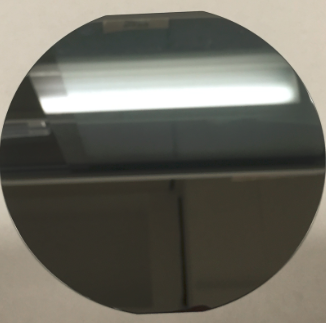
\includegraphics[height=2.5cm,width=2.5cm]{figs/experimental/plain_wafer}
		\caption[Plain wafer]{Plain, polished uncut \ch{Si}/\ch{SiO2} wafer.}
		\label{fig:plain_wafer}
	\end{minipage}
	\qquad
	\begin{minipage}[b]{0.25\linewidth}
		\centering
		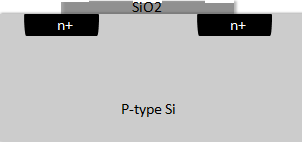
\includegraphics[height=1.75cm,width=3.25cm]{figs/experimental/si_sio2_diagram}
		\caption[Schematic of \ch{Si}/\ch{SiO2} substrate]{Schmatic of \ch{Si}/\ch{SiO2} substrate.}
		\label{fig:si_sio2_diagram}
	\end{minipage}
	\qquad
	\begin{minipage}[b]{0.25\linewidth}
		\centering
		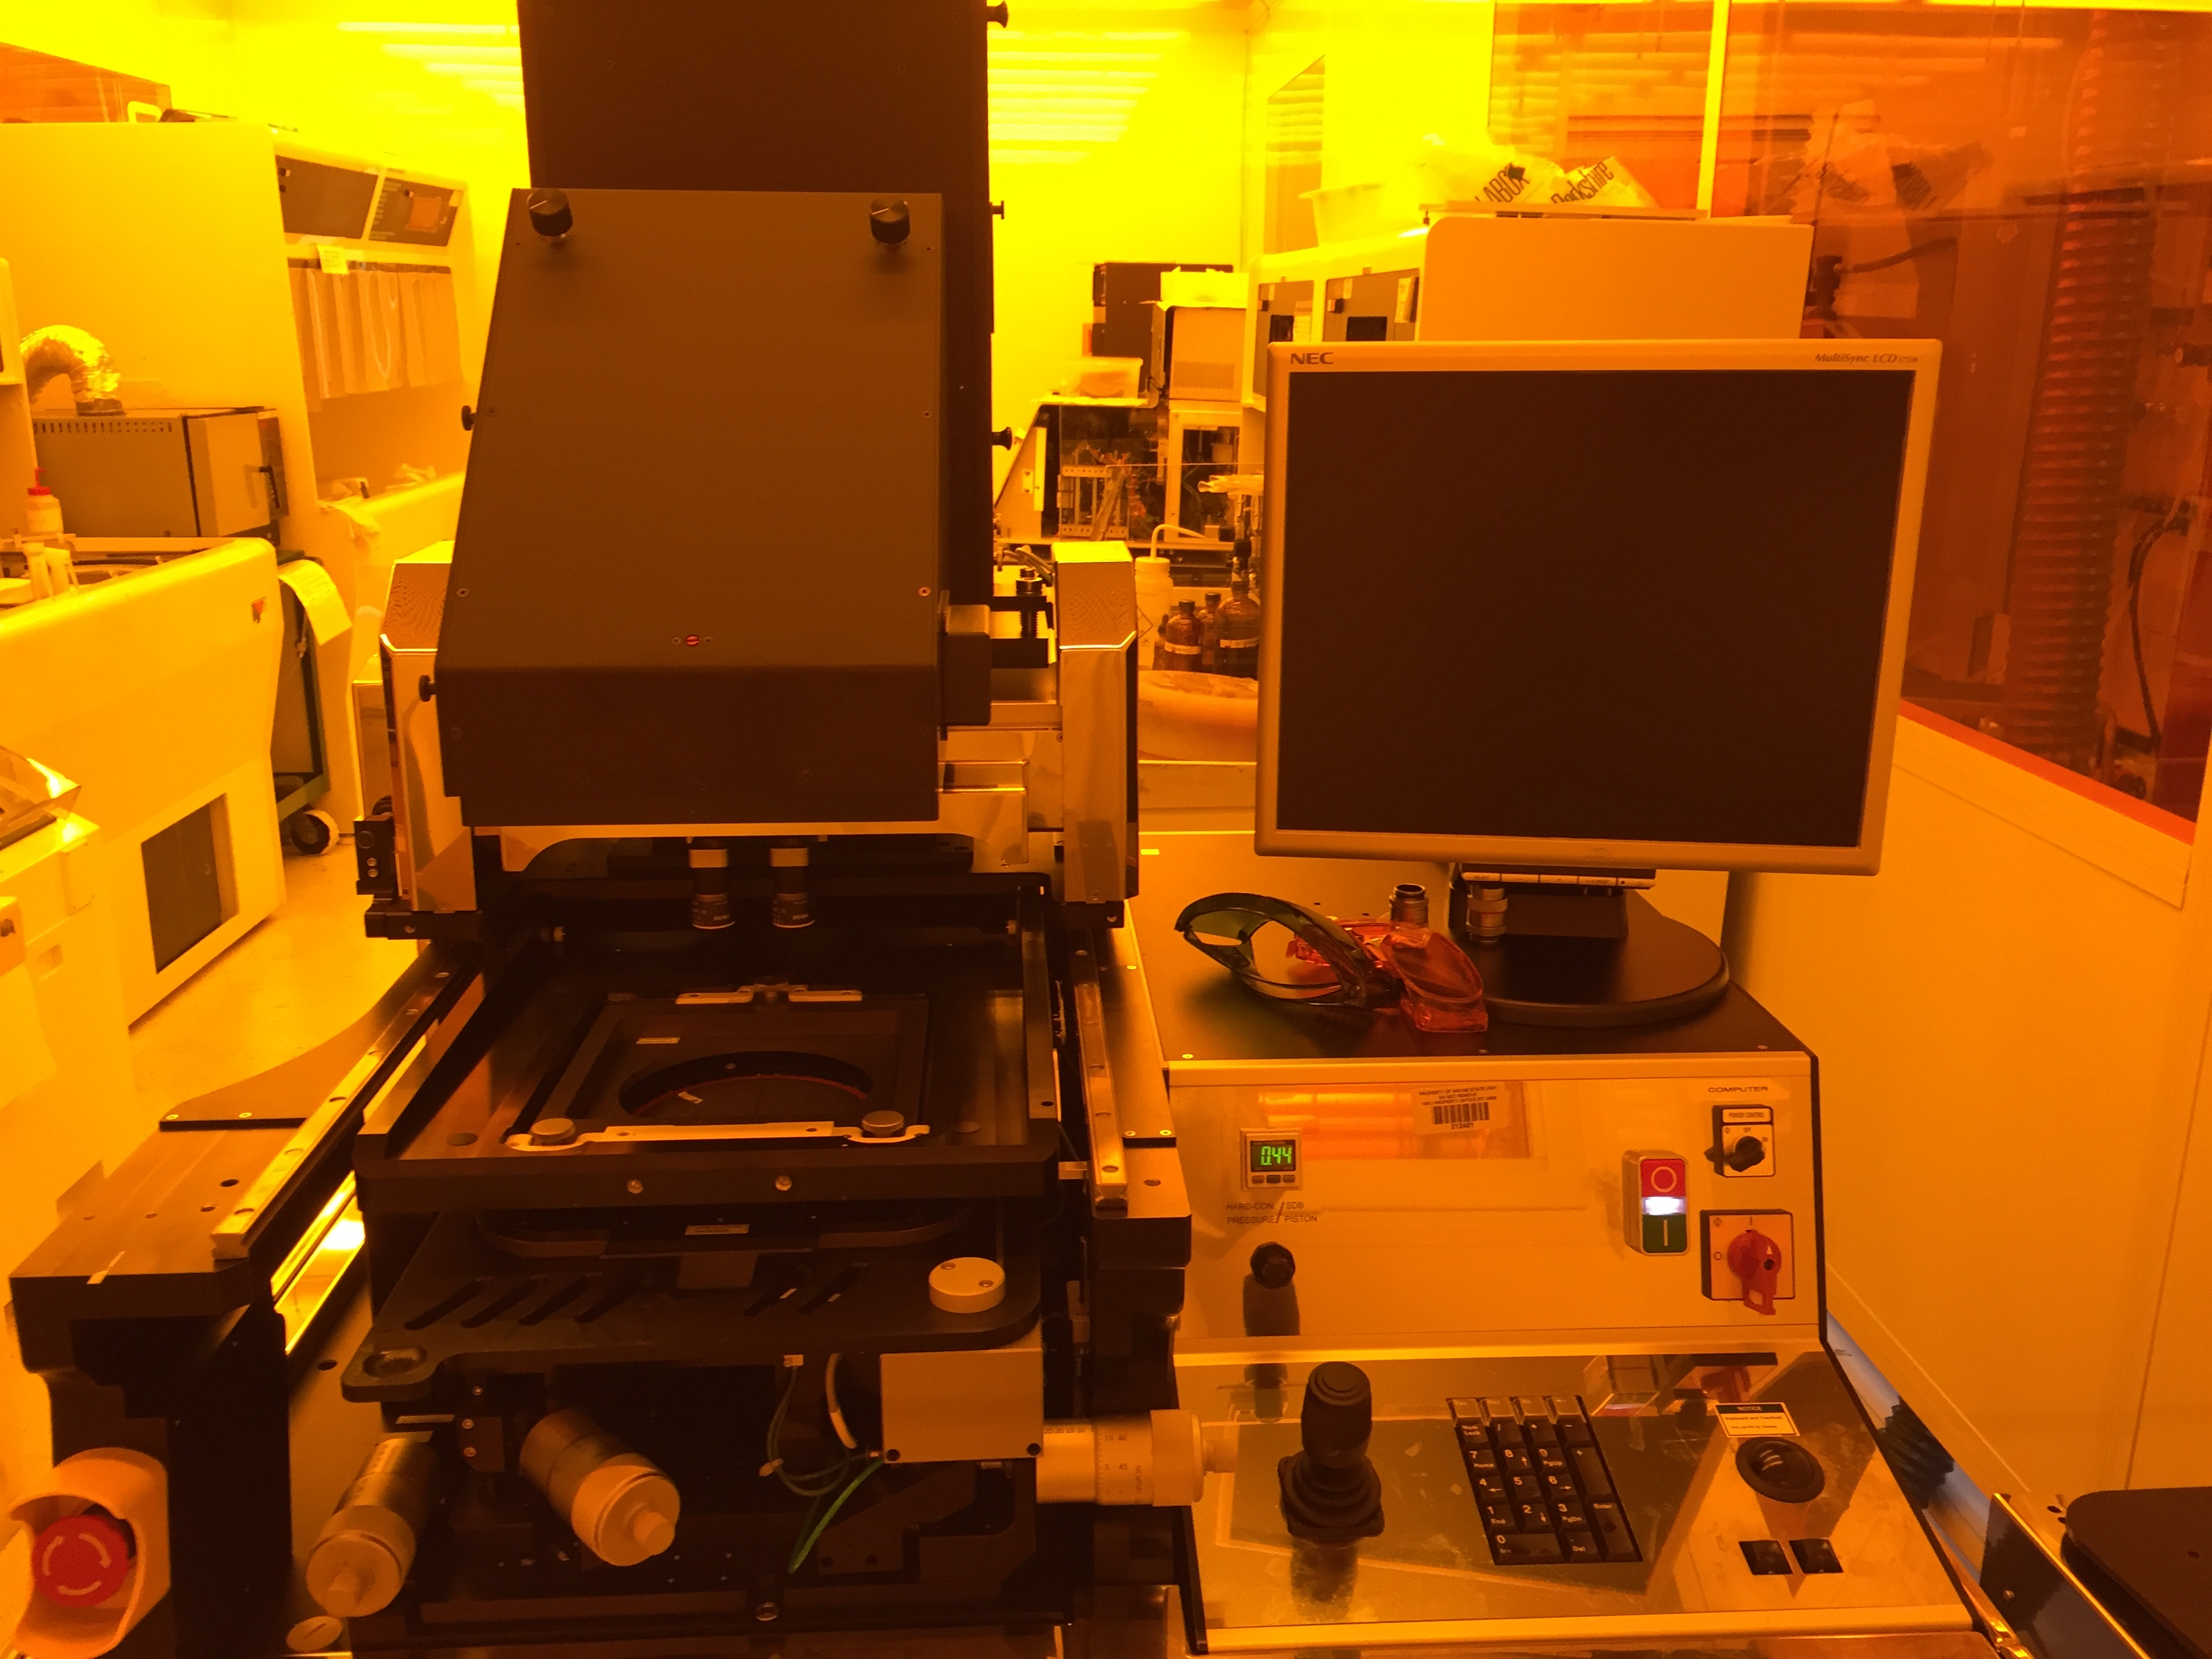
\includegraphics[height=2cm,width=3cm]{figs/experimental/photolithography_bay}
		\caption[Photolithography system]{Photolithography system for creating alignment marks on substrates.}
		\label{fig:photolithography_bay}
	\end{minipage}
\end{figure}
~

\begin{figure}[ht]
	\centering
	\subfloat[Main alignment mark at 5x magnification]{
		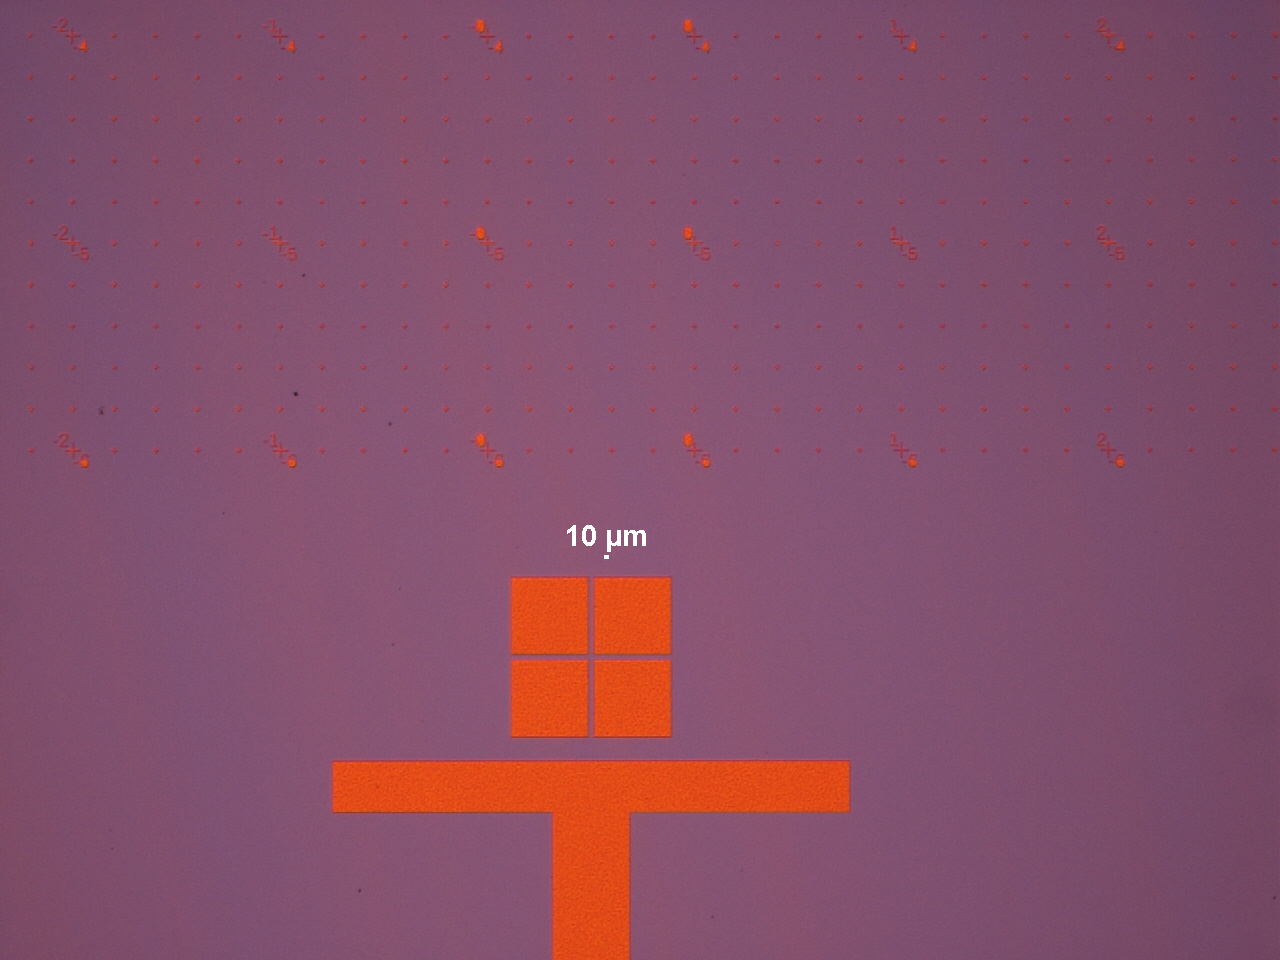
\includegraphics[height=4cm,width=5cm]{figs/experimental/main_alignment_5x}
		\label{fig:main_alignment_5x}
	}
	\qquad
	\subfloat[Main alignment mark at 10x magnification]{
		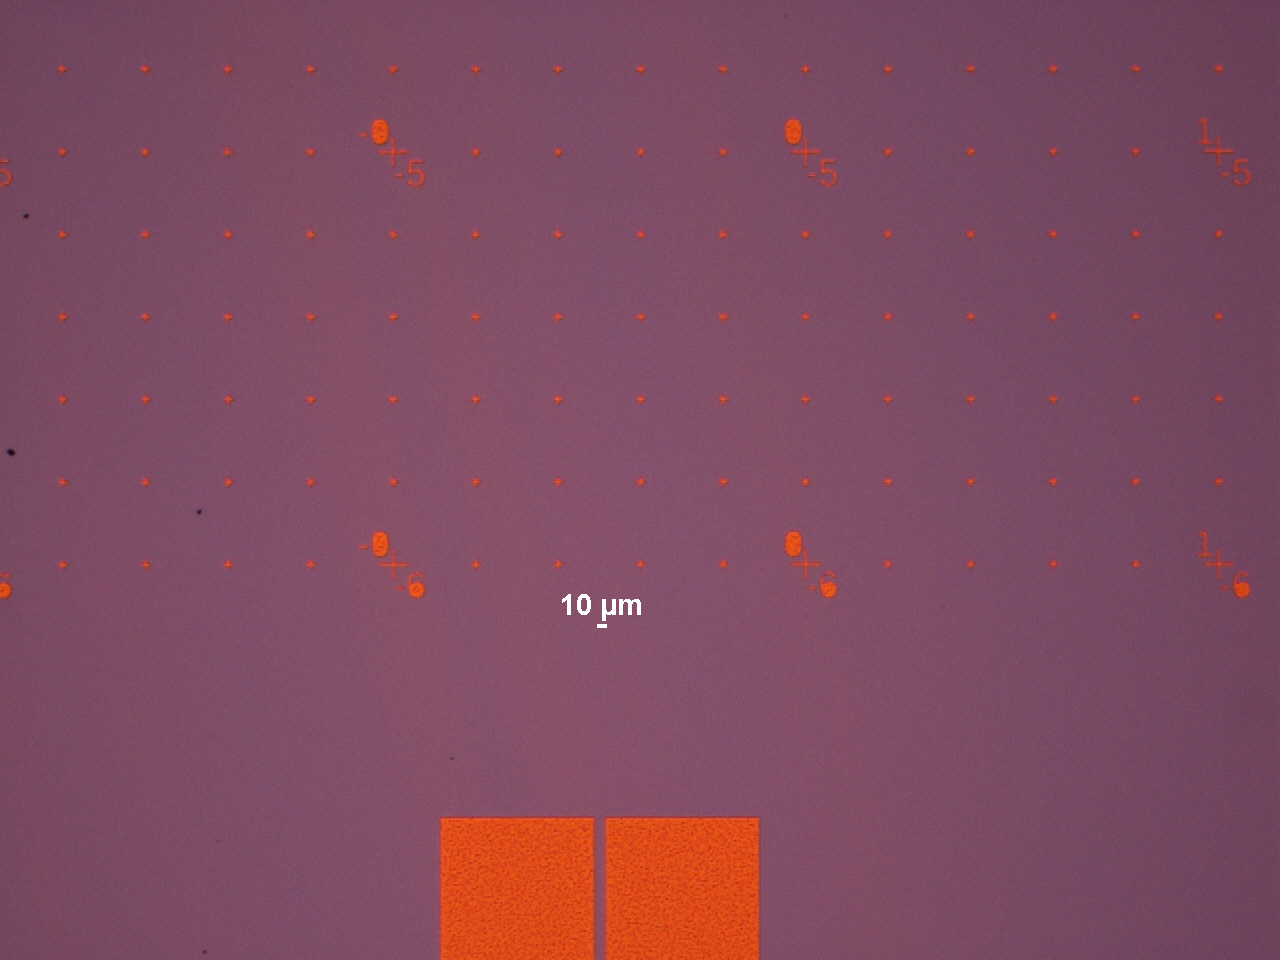
\includegraphics[height=4cm,width=5cm]{figs/experimental/main_alignment_10x}
		\label{fig:main_alignment_10x}
	}

	\subfloat[Coordinate mark $\left(0,-5\right)$ at 50x magnification]{
		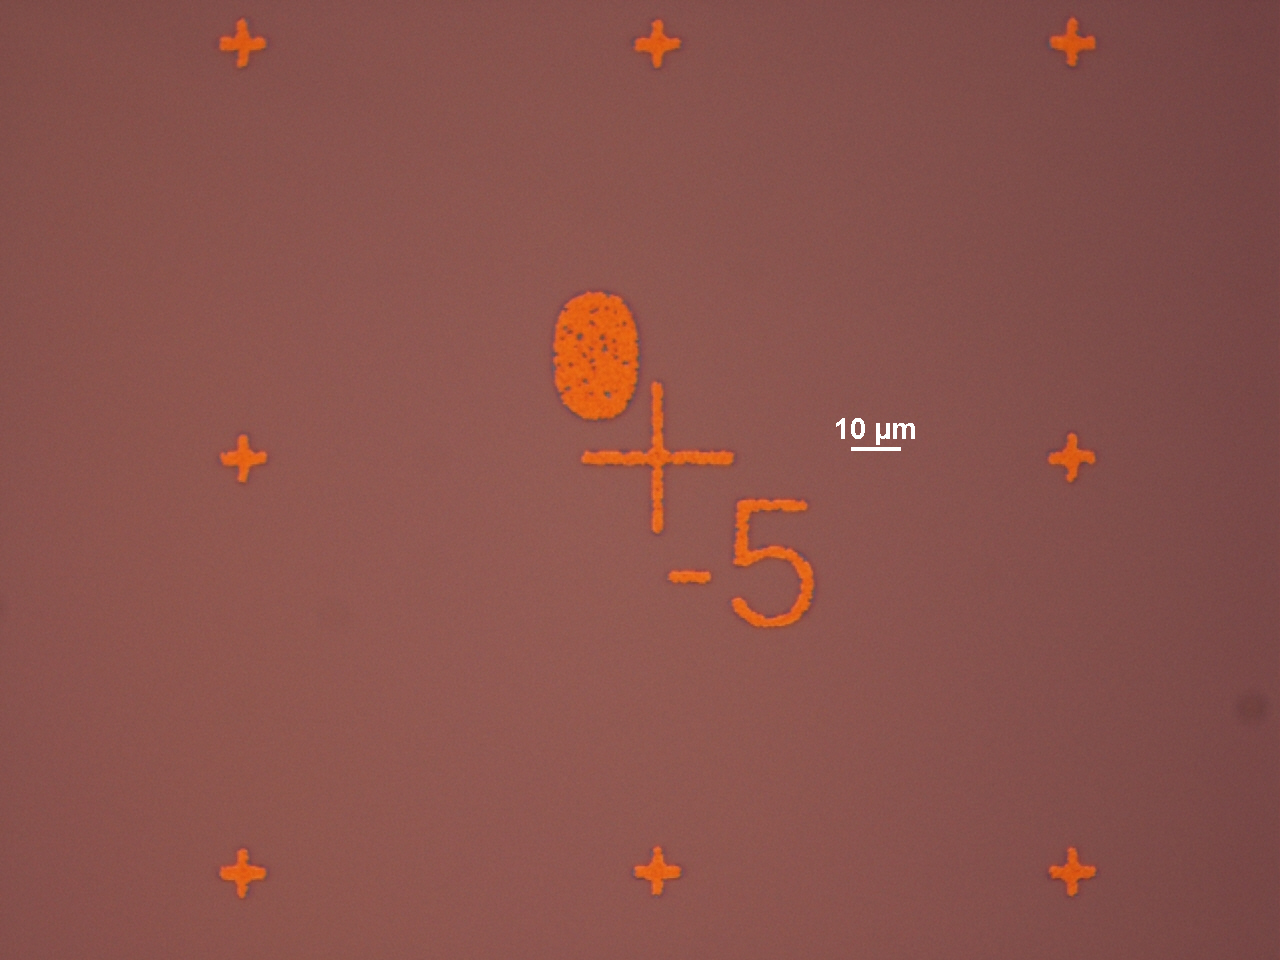
\includegraphics[height=4cm,width=5cm]{figs/experimental/main_alignment_50x}
		\label{fig:main_alignment_50x}
	}
	\qquad
	\subfloat[Coordinate mark $\left(0,-5\right)$ at 100x magnification]{
		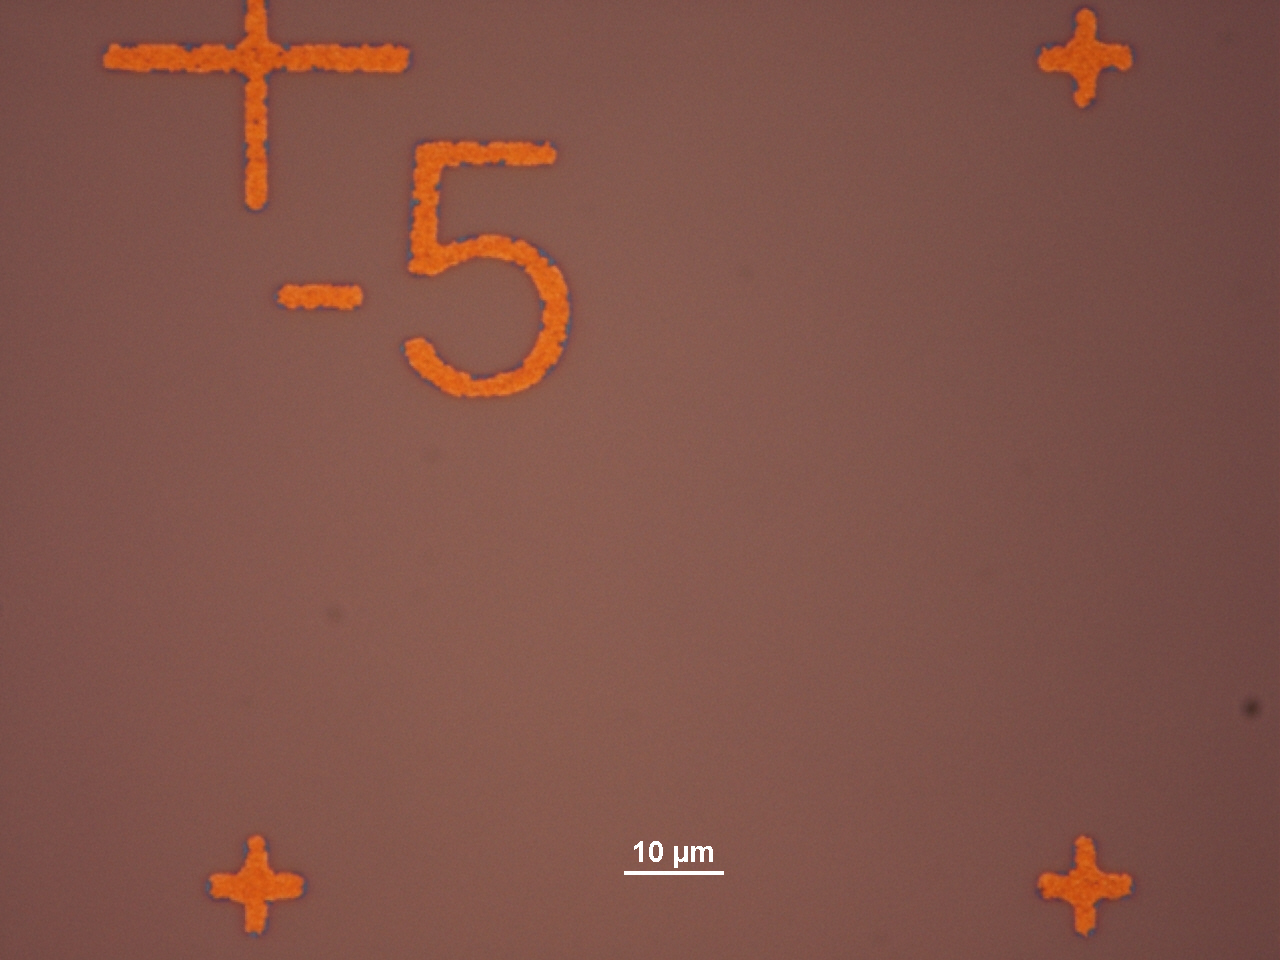
\includegraphics[height=4cm,width=5cm]{figs/experimental/main_alignment_100x}
		\label{fig:main_alignment_100x}
	}
	\caption[Alignment marks at varying magnifications]{Main alignment mark and a coordinate point on a substrate at various magnifications}
	\label{fig:main_alignment}
\end{figure}

%Testing the subref command here \subref*{fig:main_alignment_5x}, \cref{fig:main_alignment_10x}

\subsection{Substrate Cleaning}\label{subsec:cleaning}
Beginning with a cut \acs{SiO2} substrate with a deposited \acs{Au} layer. To remove the \acs{Au} layer, the substrate is first soaked in acetone for approximately 5-10 minutes then washed using \ac{IPA} and dried with \ac{N2} gas. Next, the substrate in placed in acetone and sonicated for 15 minutes. Then sonicated once more but in \acs{IPA} this time with a repition of washing and drying step using \ac{IPA} and \acs{N2} as described above in between each sonication. In order to remove and remaining organic matter on the surface of the substrate, the substrate is annealed under vacuum at $600^\degree\unita{C}$ for 10 minutes and passing forming gas for 2 of the 10 minutes. Forming gas is a mixture of \ch{H2} and an inert gas, usually \ch{N2} \cite{Choi_AppPhysLett2004}. In addition to annealing the substrate for cleanliness, in certain cases when a higher degree of cleanliness is desired the substrate can be treated with oxygen plasma cleaning. 

\section{Exfoliation}\label{sec:exfoliation}
To synthesize samples the most common and often most effective method used is mechanical exfoliation, a technique made famous by the 2004 Novoselov et al. paper. The process involves using Scotch tape to repeatedly cleave layers of \acs{MoS2} or some other TMD. Starting with a crystal of a particular TMD, placing it on a piece of Scotch tape. Then taking another piece of tape and pressing in on the crystal that is on the first piece of tape, being sure to press hard and firm on the crystal. The tape is then lifted up and this process is repeated until the whole piece of tape is filled with small samples of the TMD. At the end of this process it is expected that there are a wide range of mixture of sample sizes in terms of area and in term of thickness as well, where thicknesses of $<3\unita{nm}$ are not uncommon. To better characterize the samples the optical microscope can be used to do so.
\\ \\
\noindent The main challenge that exists with this method is the ability to synthesize a high yield of monolayer samples. This does not seem to be much of a challenge when it comes to graphene and some other TMDs, but with regard to \acs{MoS2} this is not so simple. Based on recently published literature in an effort to increase the yield of monolayer \acs{MoS2} various methods and techniques were tested and modified accordingly \cite{Huang_et_al_ACSnano2015}. In this modified method an additional step to cleaning the substrate is added in which it undergoes oxygen plasma cleaning for 10 minutes to ensure the cleanliness of the substrate`s surface. To promote more bonding between the substrate and the samples, the substrate is first heated at $300^\degree\unita{C}$ for 10 minutes without any samples on it. During this process the normal cleaving of sample on tape from crystal taking place. Once the substrate is done heating the tape containing sample is immediately placed on the substrate and pressed firmly for several minutes. Then the substrate (with the tape still on it) is placed on a glass slide (microscope slide) and is heated at around $85^\degree\unita{C}$ for five minutes. Next, the substrate (with tape) is removed from heat and the tape slowly peeled back from the substrate. The result should be a much higher yield of $<3\unita{nm}$ samples of larger surface area, and several trilayer, bilayer, and a few monolayer samples. (ADD PICTURES OF EACH STEP)
\begin{figure}[ht]
	\centering
	\subfloat[Bulk \ch{MoS2} crystal]{
		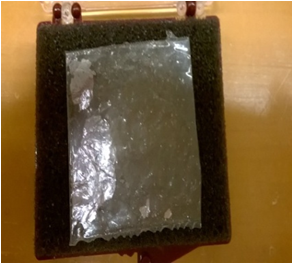
\includegraphics[height=2cm,width=3cm]{figs/experimental/exfoliation_step1}
		\label{fig:exfoliation_step1}
	}
	\qquad
	\subfloat[Single \ch{MoS2} crystal on tape]{
		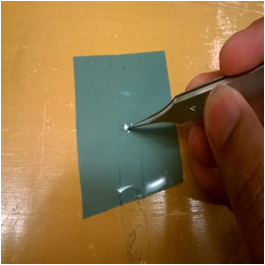
\includegraphics[height=2cm,width=3cm]{figs/experimental/exfoliation_step2}
		\label{fig:exfoliation_step2}
	}
	\qquad
	\subfloat[Tape with exfoliation \ch{MoS2} crystals]{
		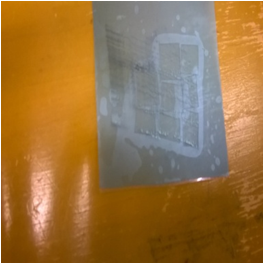
\includegraphics[height=2cm,width=3cm]{figs/experimental/exfoliation_step3}
		\label{fig:exfoliation_step3}
	}
	\caption[Exfoliation steps]{Steps of exfoliation of \ch{MoS2}.}
	\label{fig:exfoliation_steps}
\end{figure}
\\ \\
\noindent Most commonly \acs{SiO2} substrates are the main items that are exfoliated onto. However, depending on the material being synthesized, this may not always be the case. In cases where samples of \hbn or in the event that the thickness of the synthesized sample is not of great importance and can to tolerated up to $20-30\unita{nm}$, \ac{PDMS} is exfoliated onto instead of \acs{SiO2} substrates. The resulting samples are of varying thickness, on average around $20\unita{nm}$. Thin samples (usually trilayer and above) can be made using this method of \acs{PDMS}, however, these samples tend to have small surface area and lack uniformity which poses problems as to their usability. As such, this remains an effective method for obtaining samples in which thickness is not the main concern. Once the samples have been optically characterized, the sample(s) on \acs{PDMS} must be transferred to a \acs{SiO2} substrate.

\section{Device Synthesis}\label{sec:synthesis}
Once the sample or samples have been synthesized and characterized for their specific purpose these samples can begin to be synthesized into a device for measurement. Generally, this involves the technique of transfer. Transfer is usually done using the aforementioned \acs{PDMS} or using \ac{PC} known as the \acs{PC} pickup method. Each method has its advantages and disadvantages depending on the type of sample, type of device, or any number of the factors.
%
\subsection{\acs{PDMS} Transfer}\label{subsec:pdms_transfer}
\acs{PDMS} transfer is most useful for samples that were originally exfoliated onto \acs{PDMS}, for example \hbn. To manufacture \acs{PDMS} a 10:1 ratio of silicone base and curing agent is mixed together and placed in vacuum for 30 minutes to ensure the removal of any remaining air bubbles. After this time the mixture is then spin coated on a plain \acs{SiO2} wafer and heated at $80^\degree\unita{C}$ for 30 minutes then allowed to cool for 30 minutes. Once cooled, the surface of the wafer can be cut using a razor into small stamps that can used for exfoliation and for transfer. \\ \\
\noindent Once the samples that are to be transferred are on the \acs{PDMS} stamp, then it is placed on a glass slide. Using the optical microscope to locate the sample on the stamp and using a razor to cut small excess pieces from the portions of the stamp where the desired sample is not located. This process is repeated until the size of the cut stamp is now reasonably small. The cut stamp is then placed at the edge of a new glass slide with sample area of the stamp as close to the edge as can be and the other side of the stamp is taped down using Scotch tape. \\ \\
\noindent Next a substrate is placed and secured using glue (usually PMMA) to the stage of the transfer setup. The transfer stage setup is pictured in fig.~\ref{fig:transfer_stage_setup}. It consists of a microscope that has the capability of 10x or 20x magnification and a micro-manipulator. The micro-manipulator is where the glass slide with the \acs{PDMS} stamp is placed. Using the manipulator the substrate on the stage is approached and the position of the stamp is checked and re-checked multiple times using the microscope to ensure correct overlap of the desired portion of the sample(s). Upon reaching the desired position, the glass slide is lowered but this time there should be a contrast seen which is the overlapping of the glass slide and the substrate. Once the contrast has enveloped the entire sample that was to be transferred then the manipulator can be used to lift up the glass slide. Once the transfer is complete then the substrate should be annealed at $250^\degree\unita{C}$ for 30 minutes in order to remove and residue or orgranic matter that may have remained during the transfer process.
\begin{figure}[ht]
	\centering
	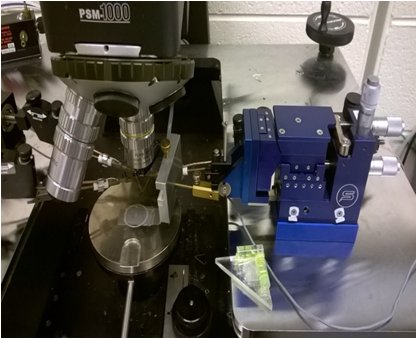
\includegraphics[height=5cm,width=5cm]{figs/experimental/transfer_stage_setup}
	\caption[Transfer stage setup]{Transfer stage setup}
	\label{fig:transfer_stage_setup}
\end{figure}
\subsection{Polycarbonate Pickup Method}\label{subsec:pc_pickup}
The PC pickup method is used for samples that have been exfoliated onto a \acs{SiO2} substrate. Generally these are thinner samples with larger surface area that are not as easily obtained by using the PDMS exfoliation method as described in sec.~\ref{sec:exfoliation}. To manufacture the PC, $3.0\unita{g}$ of chloroform and $0.18\unita{g}$ of polycarbonate resin are put on a plate shaker for about 60 minutes or until the polycarbonate resin have dissolved into the solution. \\ \\
\noindent Next, the substrate that has the sample that is going to be transferred in taped using double-sided tape to a glass slide facing up. Then using a syringe the \acs{PC} solution is placed in the substrate and evenly spread across it. Being sure to locate the area(s) on the substrate where the sample(s) are located, small pre-cut pieces of PDMS are placed over top of these areas. An outline of the \acs{PDMS} stamps is cut using a razor and any excess \acs{PDMS} is carefully torn away. Once only the \acs{PDMS} strips are remaining on the substrate \ac{DI} is put under the strips in order to create a hydrophobic surface and to ensure that the strip and PC that is trapped underneath it come off the substrate with relative ease. Each strip is placed on its own glass slide and is gently blown with \ch{N2} gas to remove any excess \acs{DI} from the surface. \\ \\
\noindent Moving to the transfer stage setup and following the steps described in sec.~\ref{subsec:pdms_transfer} with regard to using the transfer stage setup. The only difference at this point to using this method as opposed to \acs{PDMS} transfer is in the final step of the transfer. Instead of only lowering until the contrast change is shown between the region that is desired to be transferred, with PC transfer the entire PC must be lowered down. This is because since the PC will be heated before being lifted up. Lowering all the way ensures that all the PC will be melted. Once lowered all the way, the heating device, which is connected to the stage, should be turned up to $130^\degree\unita{C}$. Once this temperature is reached, it should be maintained for approximately two minutes to fully melt the PC film. After heating the substrate and lifting up using micro-manipulator the substrate is placed in chloroform and covered for 30-60 minutes. The purpose of this is to remove any residue left over by the PC film or any other items that may have been introduced at any point in the transfer process. In practice the chloroform soaking generally needs to be repeated several times over a few hours in order to ensure the least amount of remaining residue possible. To confirm the reduction of residue and also characterize the transferred samples an AFM is used. 

\section{Characterization}\label{sec:characterization}
There are many ways used in modern academia and industry to characterize samples and devices. Some of these methods include \ac{STM}, \ac{TEM}, \ac{AFM}, and \ac{MFM} \cite{Kittel_IntroSolidState2005}. The primary characterization techniques used in this project are \acs{AFM} and optical characterization.
\subsection{Optical Characterization}\label{subsec:characterization_optical}
The majority of the optical characterization is carried out using the optical microscope as shown in figs.~\ref{fig:optical_microscope_front_view} and~\ref{fig:optical_microscope_side_view}. The microscope can magnify 5x, 10x, 20x, 50x, and 100x, in addition, it can show dark field images.
\begin{figure}[ht]
	\centering
	\begin{minipage}[b]{0.45\linewidth}
		\centering
		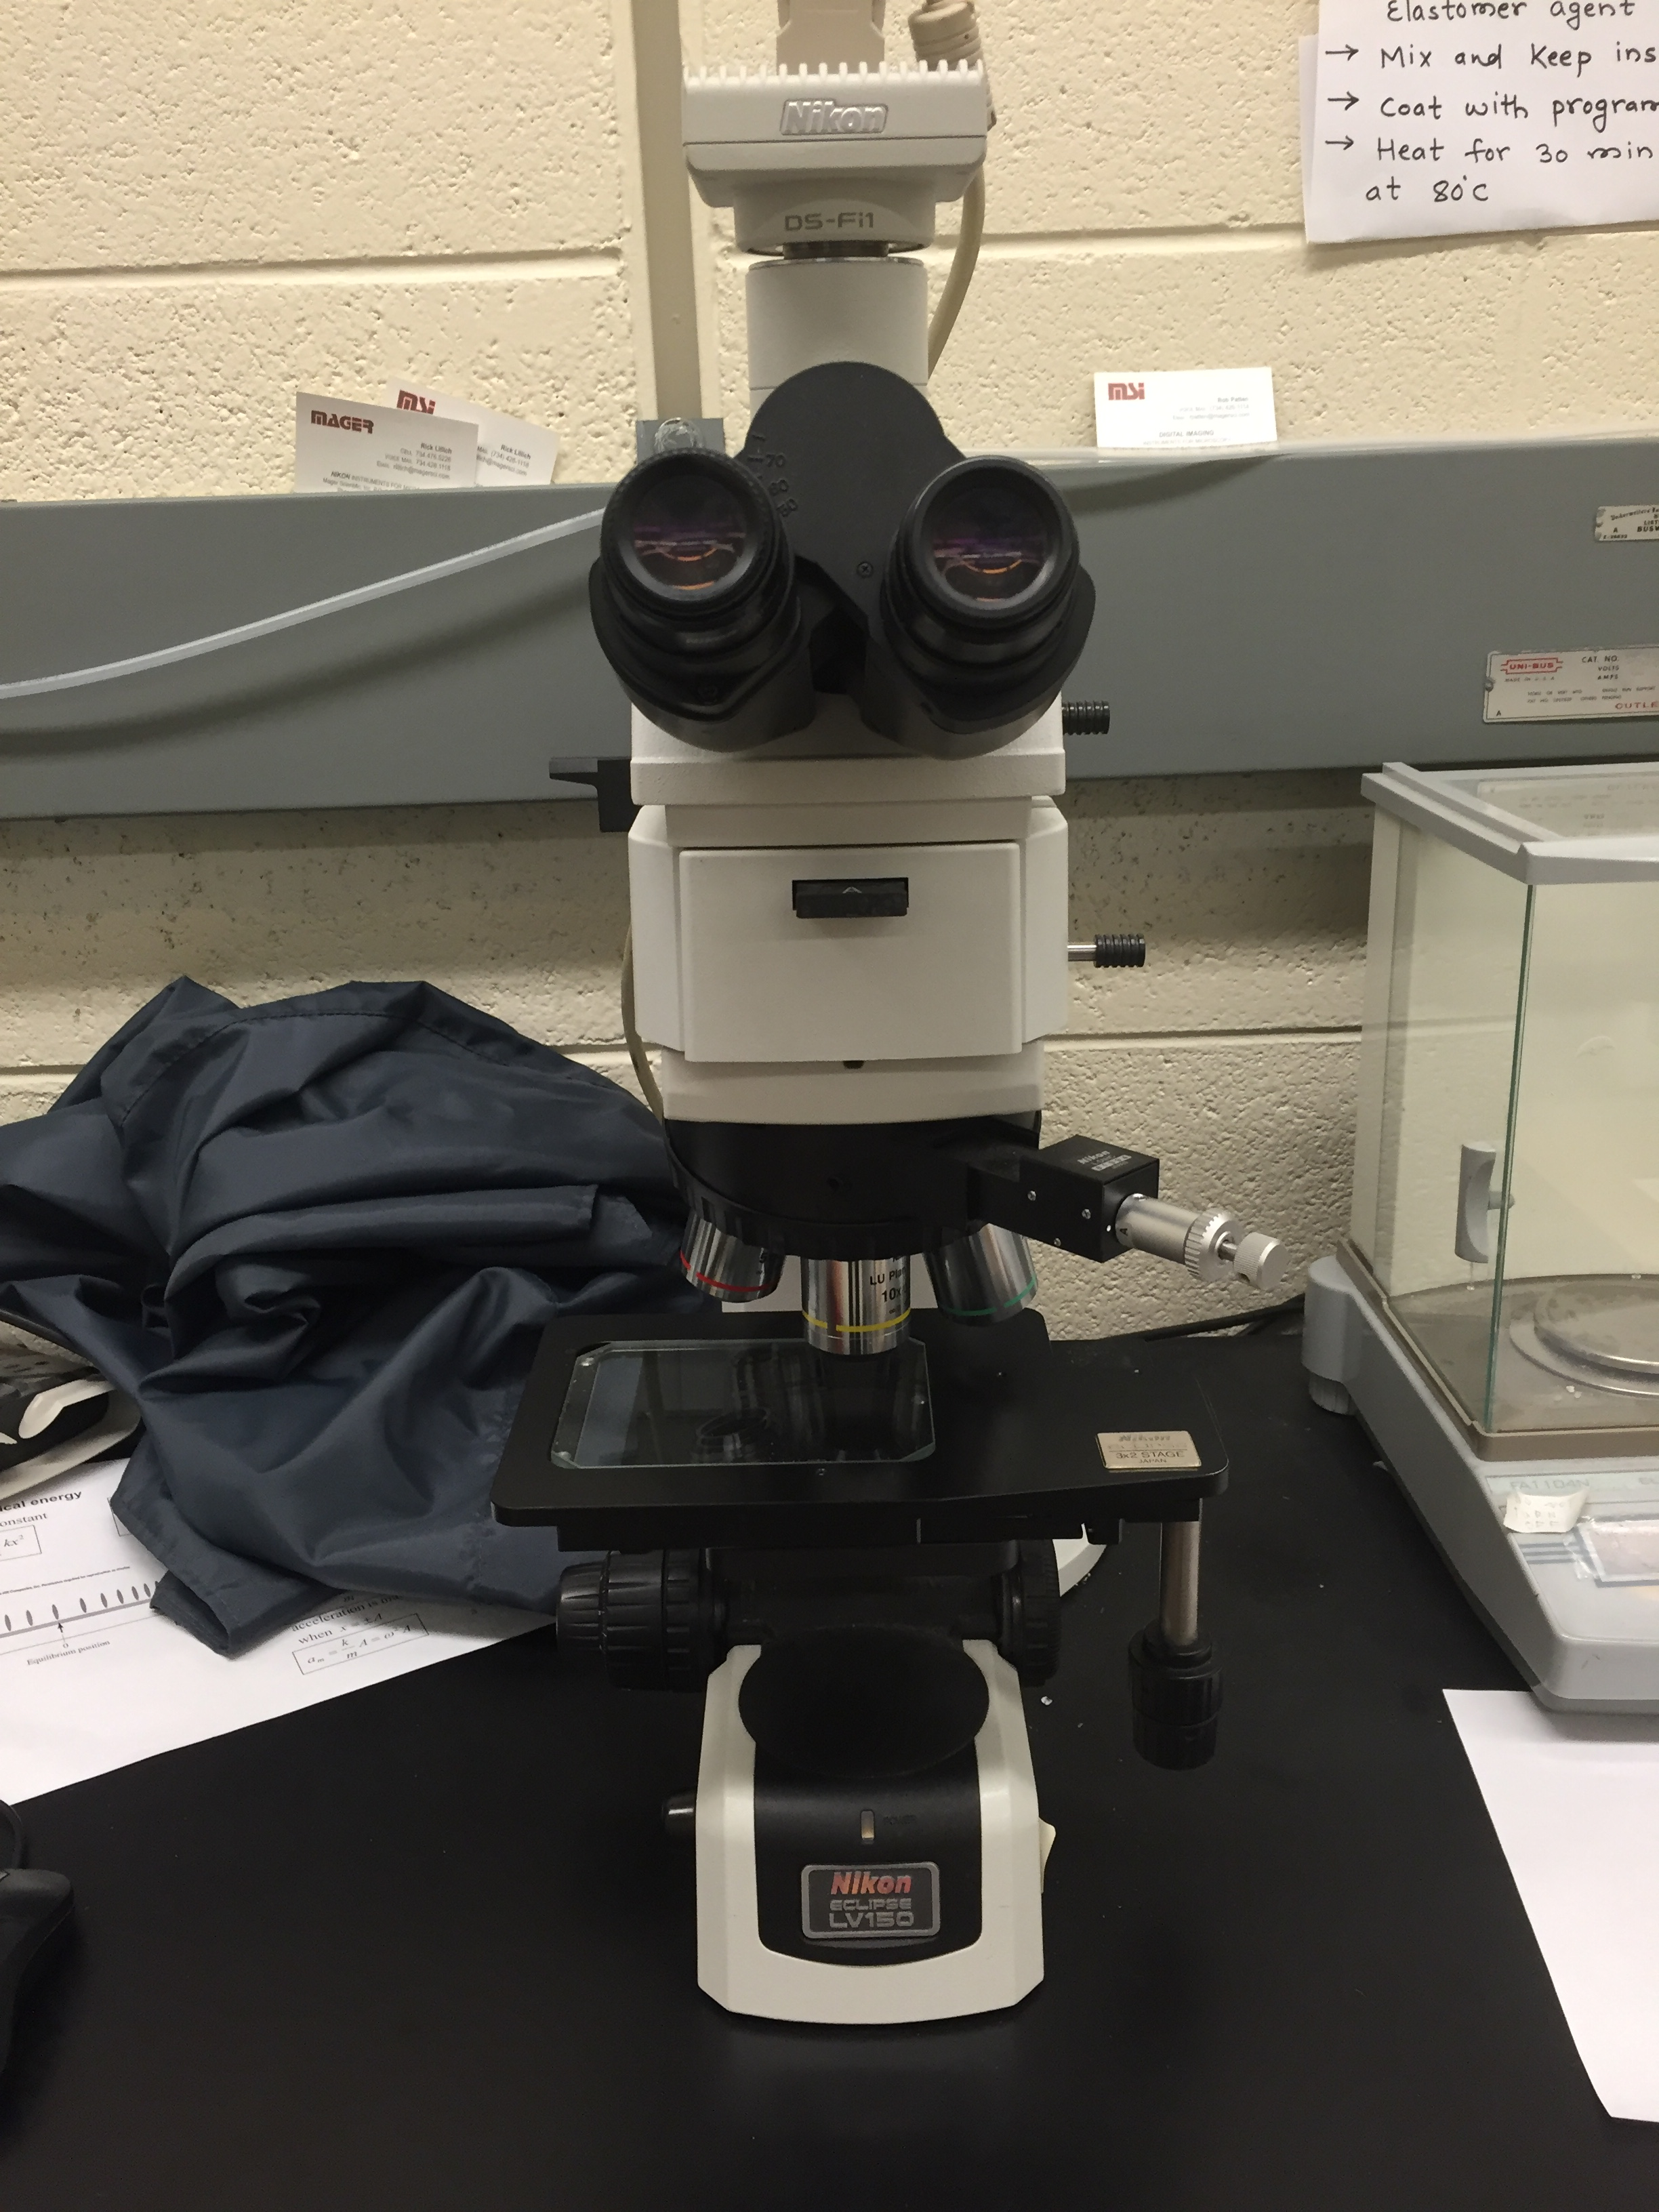
\includegraphics[height=5cm,width=5cm]{figs/experimental/optical_microscope_front_view}
		\caption[Optical microscope front view]{Optical microscope front view}
		\label{fig:optical_microscope_front_view}
	\end{minipage}
	\qquad
	\begin{minipage}[b]{0.45\linewidth}
		\centering
		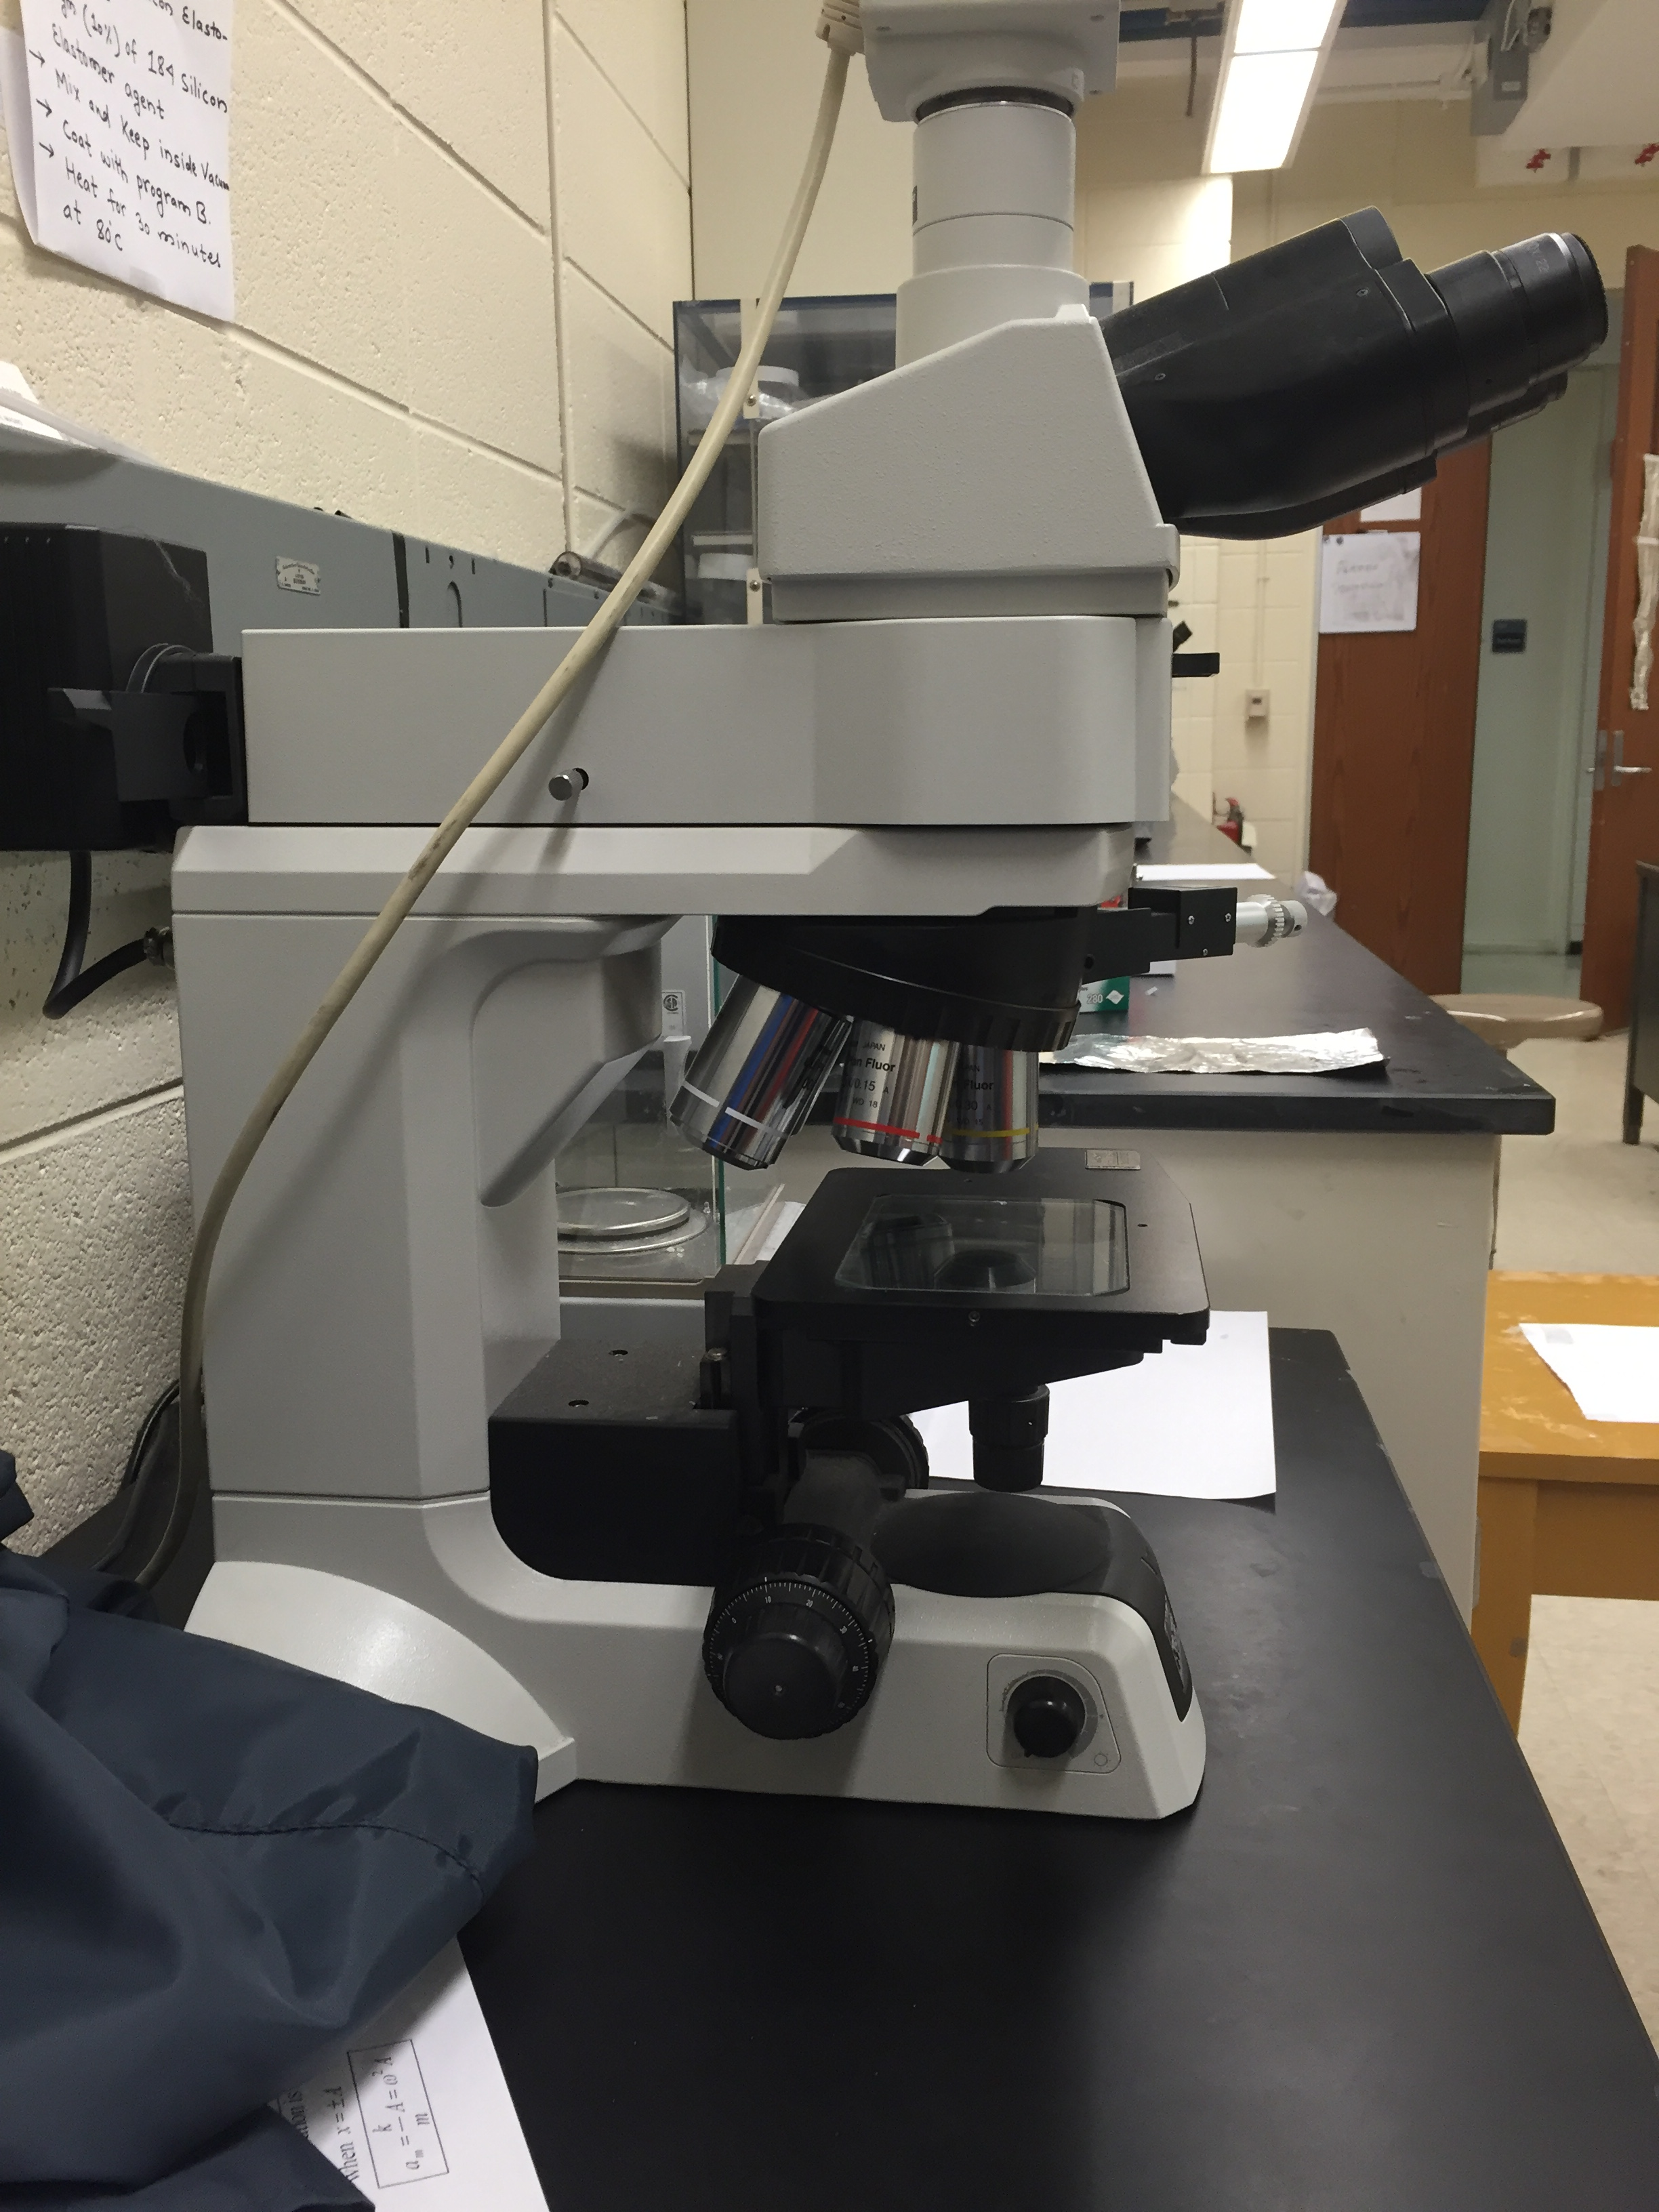
\includegraphics[height=5cm,width=5cm]{figs/experimental/optical_microscope_side_view}
		\caption[Optical microscope side view]{Optical microscope side view}
		\label{fig:optical_microscope_side_view}
	\end{minipage}
\end{figure}

\subsection{AFM Characterization}\label{subsec:characterization_afm}
In addition to the characterizing samples optically, \acs{AFM} characterization is another important aspect of the device design and fabrication process. \acs{AFM} characterization occurs several times throughout the process, after each transfer of a sample onto another, for example. This occurs for two reasons; to verify the thickness of the sample(s) that have been transferred, and also to verify the cleanliness of the surface of the sample (to ensure that any residue has been removed, especially during the course of PC transfer). Additionally, once the electrodes of the device have been fabricated a final \acs{AFM} characterization is need to determine the width of the device`s channel which is needed to calculate various important electrical properties. \\ \\

\noindent Fig.~\ref{fig:afm_front_view} shows a front view of the \acs{AFM} used to characterize. For these purposes, the \acs{AFM} is operating in ``tapping" mode which is less invasive than ``contact" mode \cite{Kittel_IntroSolidState2005}. In basic terms, an \acs{AFM} works by measuring the force between the tip of a cantilever (see fig.~\ref{fig:AFM_tip}) and the sample being imaged. 
\begin{figure}[ht]
	\centering
	\begin{minipage}[b]{0.45\linewidth}
		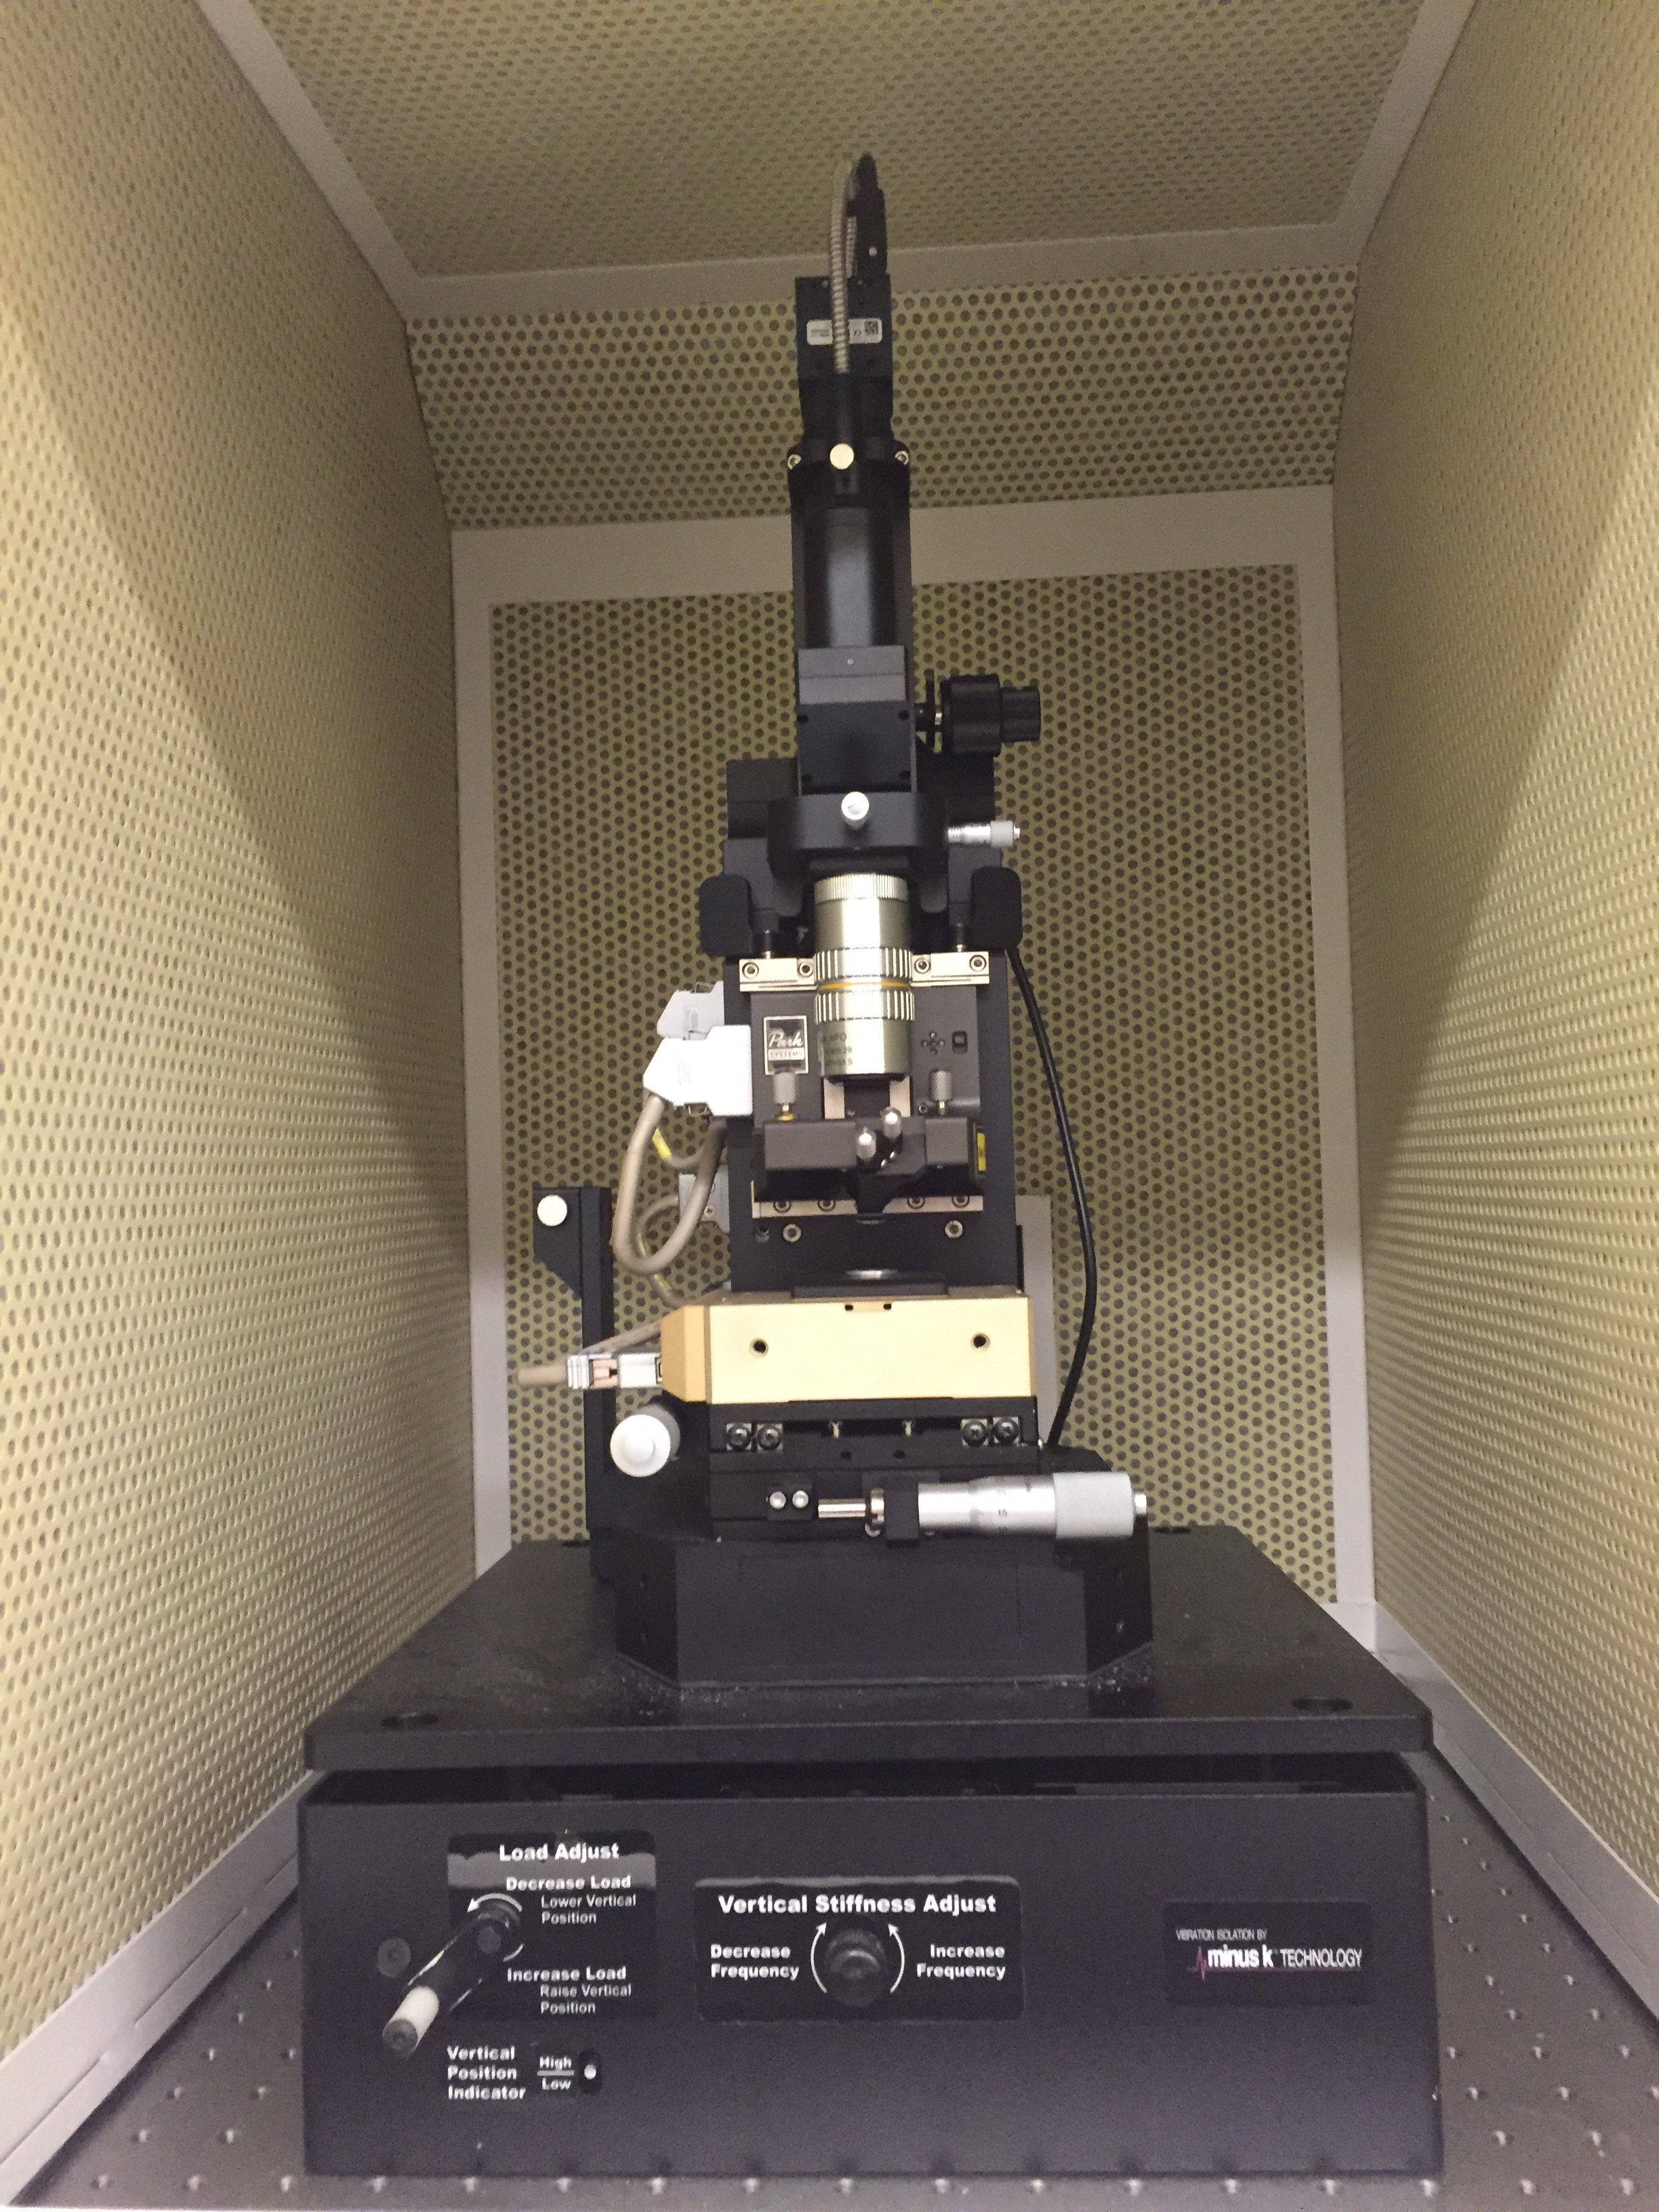
\includegraphics[height=4cm,width=4cm]{figs/experimental/AFM_front_view}
		\caption[AFM front view]{AFM front view}
		\label{fig:afm_front_view}
	\end{minipage}
	\qquad
	\begin{minipage}[b]{0.45\linewidth}
		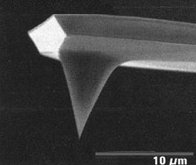
\includegraphics[height=4cm,width=4cm]{figs/experimental/AFM_tip}
		\caption[AFM cantilever]{AFM cantilever \cite{Ernst-Moritz-Arndt_Online}}
		\label{fig:AFM_tip}
	\end{minipage}
\end{figure}

\section{Device Fabrication}\label{sec:device_fabrication}
\subsection{Device Design}\label{subsec:device_design}
\subsection{Electron Beam Lithography}\label{subsec:lithography}
\begin{figure}[ht]
	\centering
	\includegraphics[height=3cm,width=5cm]{figs/experimental/SEM}
	\caption[Scanning electron microscope]{Control panel and electron beam writer of scanning electron microscope.}
	\label{fig:SEM_machine}
\end{figure}

\begin{figure}[ht]
	\centering
	\subfloat[Developed pattern 10x]{
		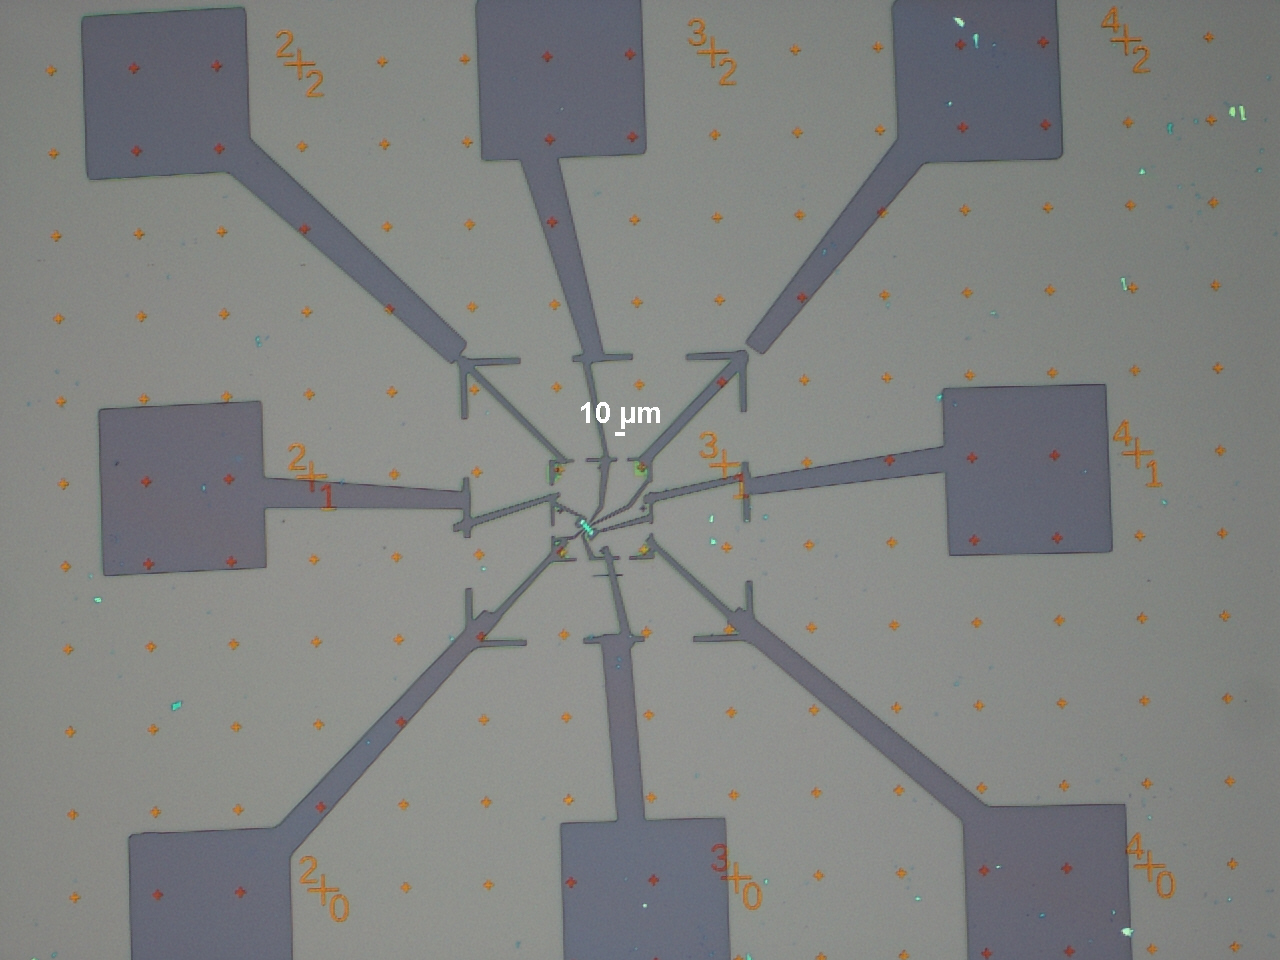
\includegraphics[height=4cm,width=4cm]{figs/experimental/ebeam_developed_10x}
		\label{fig:ebeam_developed_10x}
	}
	\qquad
	\subfloat[Developed pattern 100x]{
		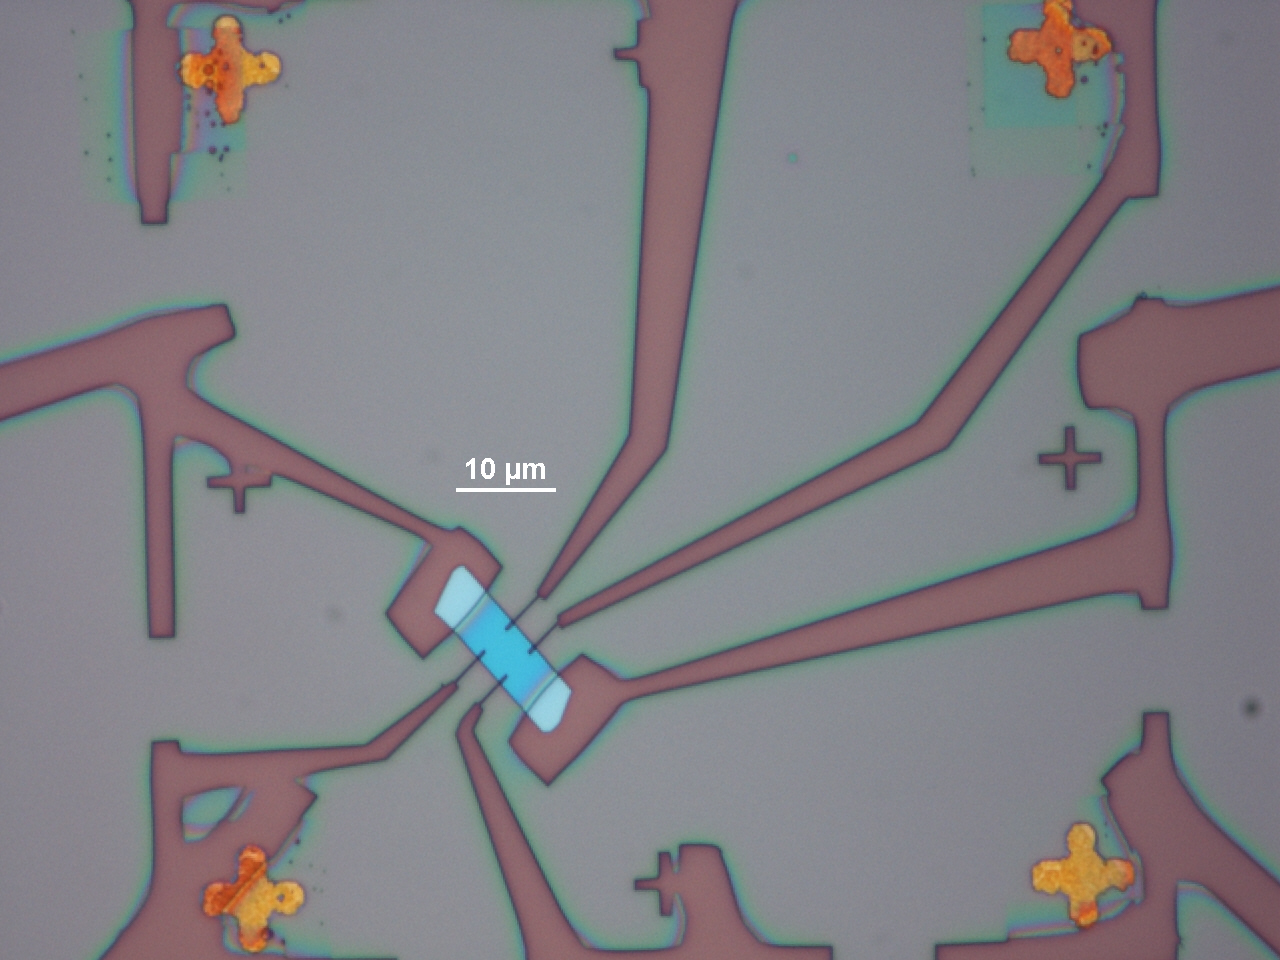
\includegraphics[height=4cm,width=4cm]{figs/experimental/ebeam_developed_100x}
		\label{fig:ebeam_developed_100x}
	}
	\caption[Electron beam lithography patterns]{10x and 100x electron beam lithography patterns developed using \acs{MIBK} and \acs{MEK}.}
	\label{fig:ebeam_developed}
\end{figure}

\subsection{Metal Deposition}\label{subsec:deposition}
\begin{figure}[ht]
	\centering
	\begin{minipage}[b]{0.45\linewidth}
		\centering
		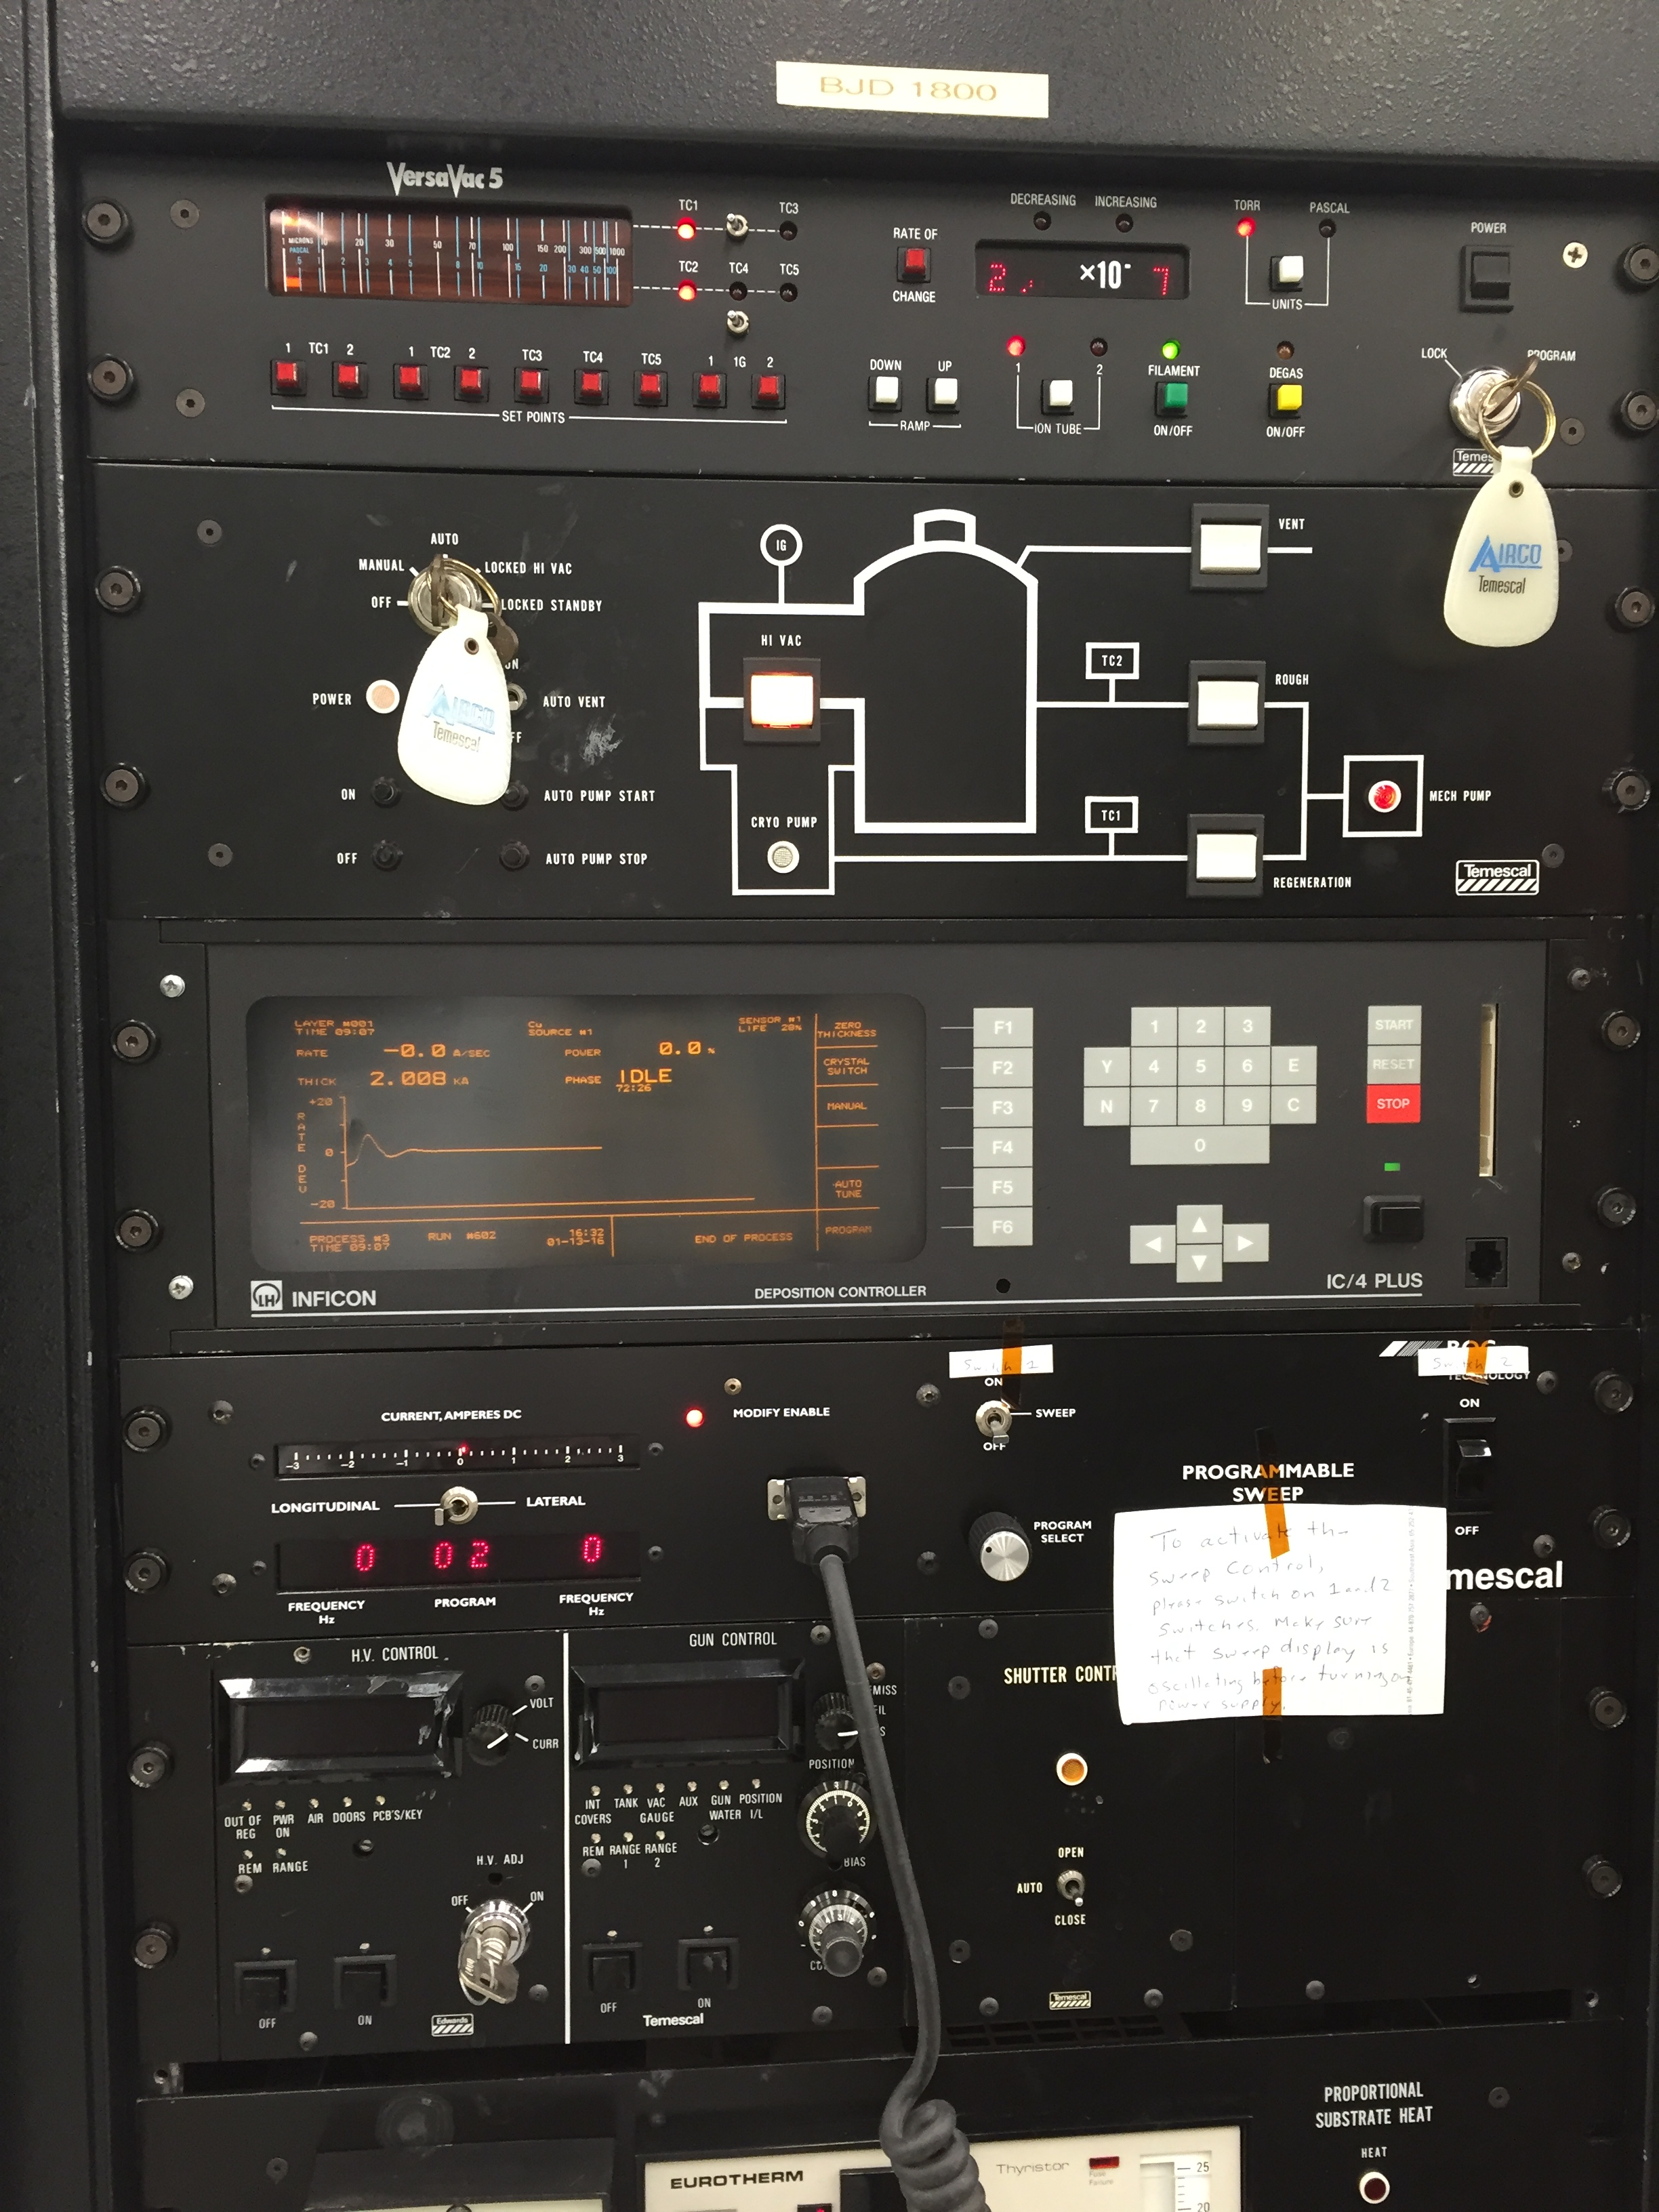
\includegraphics[height=4cm,width=4cm]{figs/experimental/bjd_control_panel}
		\caption[BJD control panel]{caption 1}
		\label{fig:bjd_control_panel}
	\end{minipage}
	\qquad
	\begin{minipage}[b]{0.45\linewidth}
		\centering
		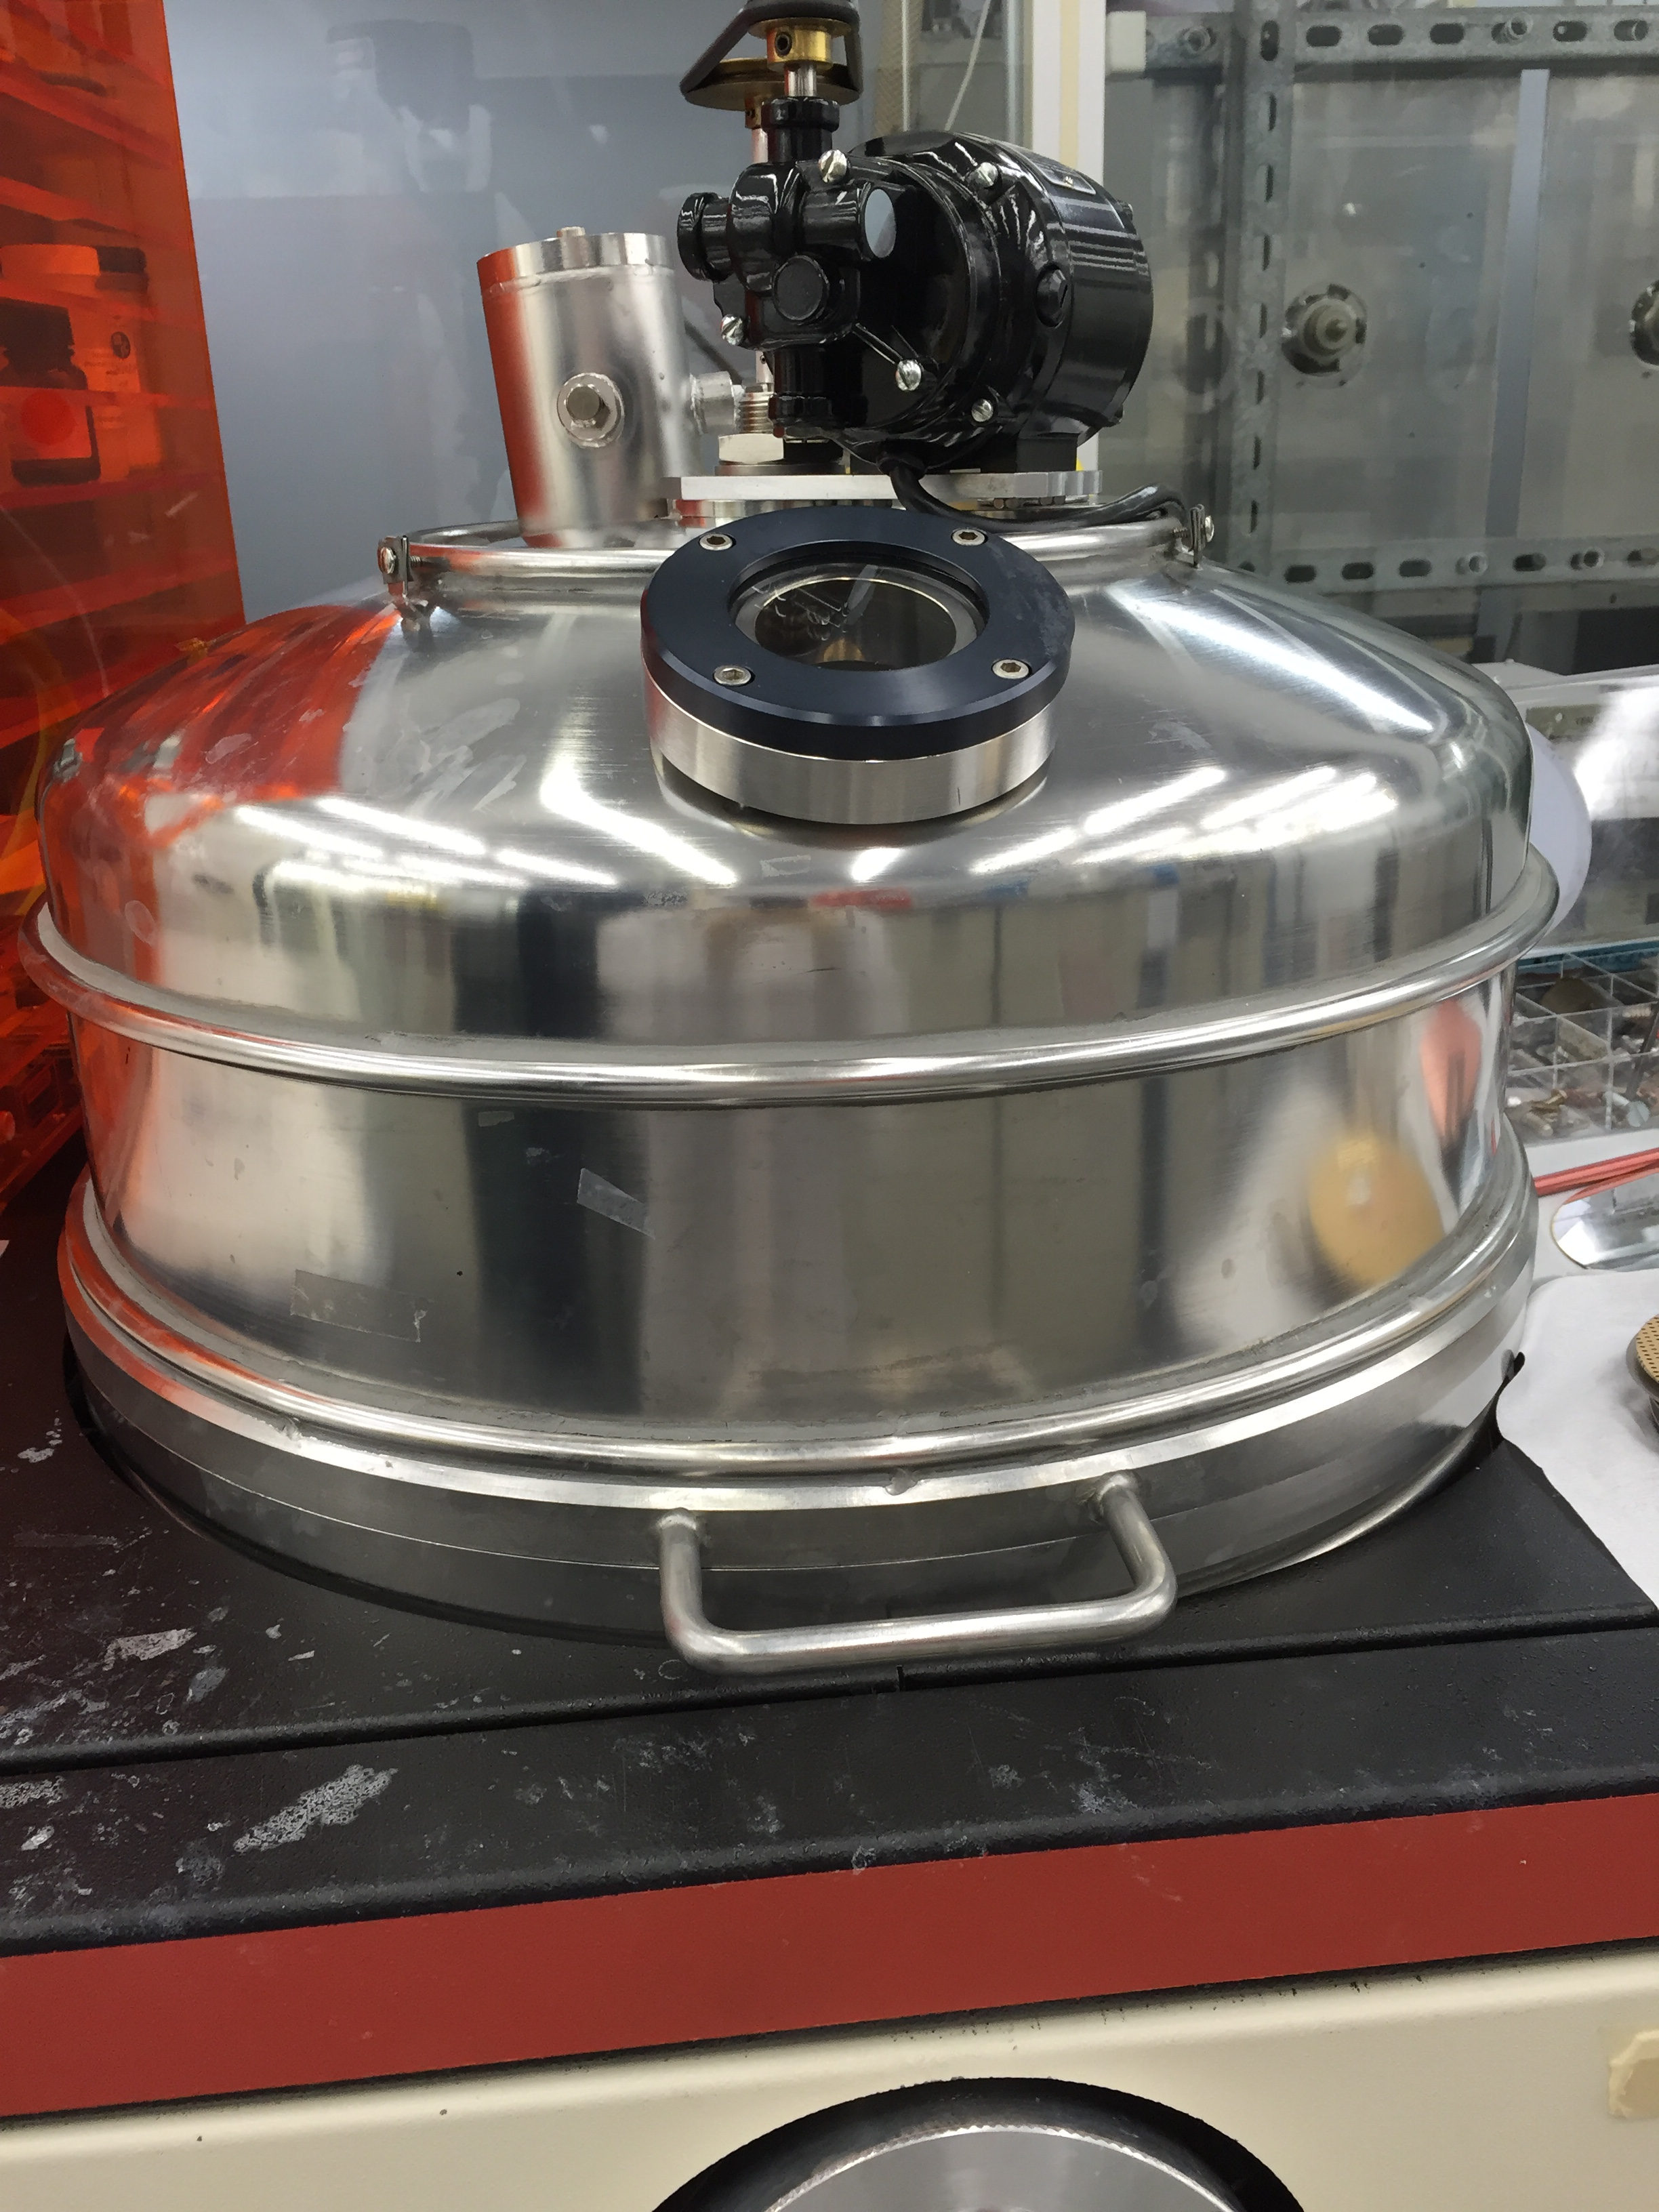
\includegraphics[height=4cm,width=4cm]{figs/experimental/bjd_hood}
		\caption[BJD Hood]{caption 2}
		\label{fig:bjd_hood}
	\end{minipage}
\end{figure}

\begin{figure}[ht]
	\centering
	\subfloat[\ch{Au}/\ch{Ti} deposited on developed sample after electron beam lithography at 10x]{
		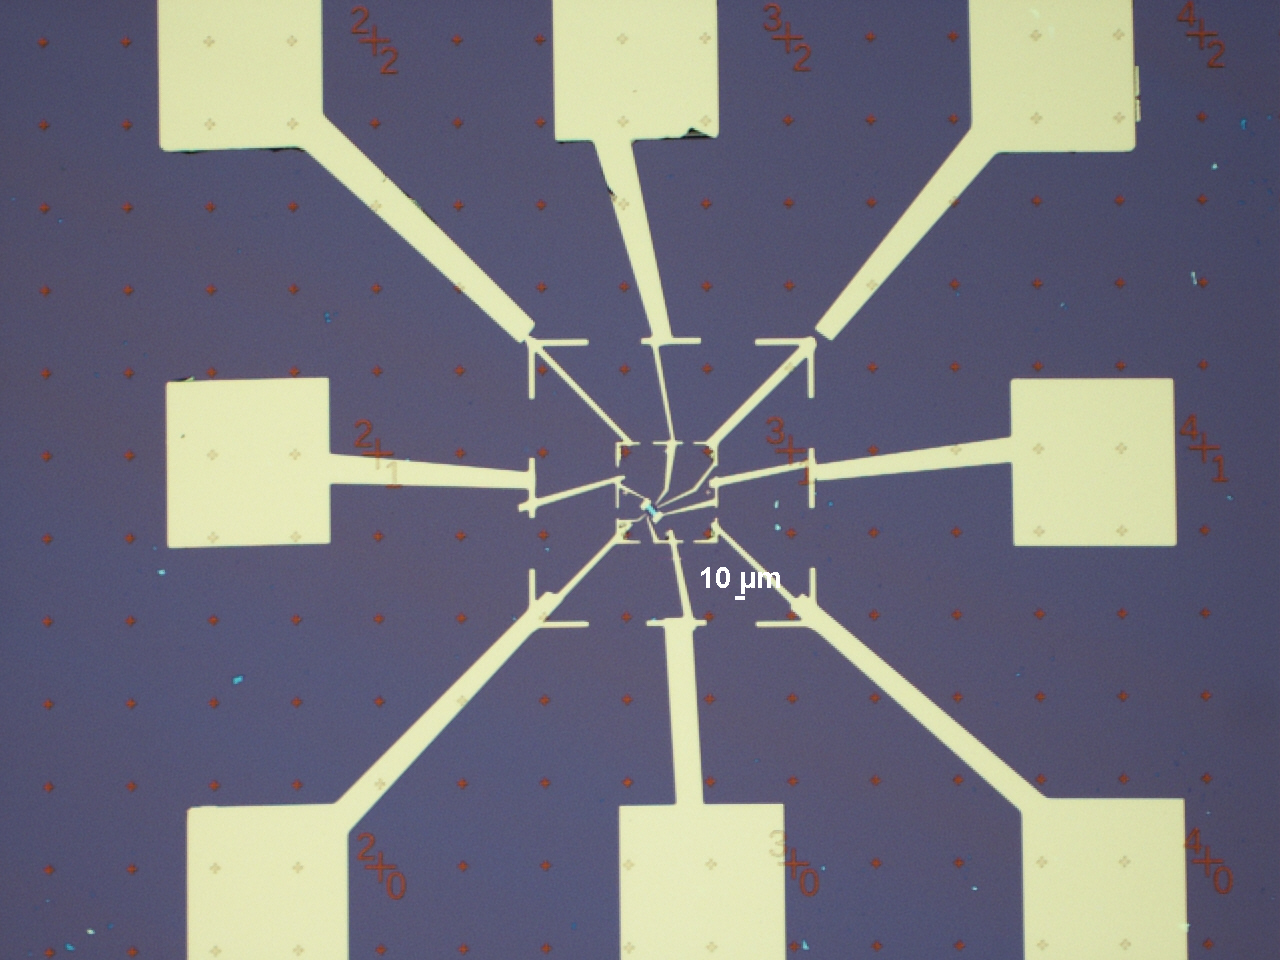
\includegraphics[height=4cm,width=4cm]{figs/experimental/liftoff_10x}
		\label{fig:liftoff_10x}
	}
	\qquad
	\subfloat[\ch{Au}/\ch{Ti} deposited on developed sample after electron beam lithography at 100x]{
		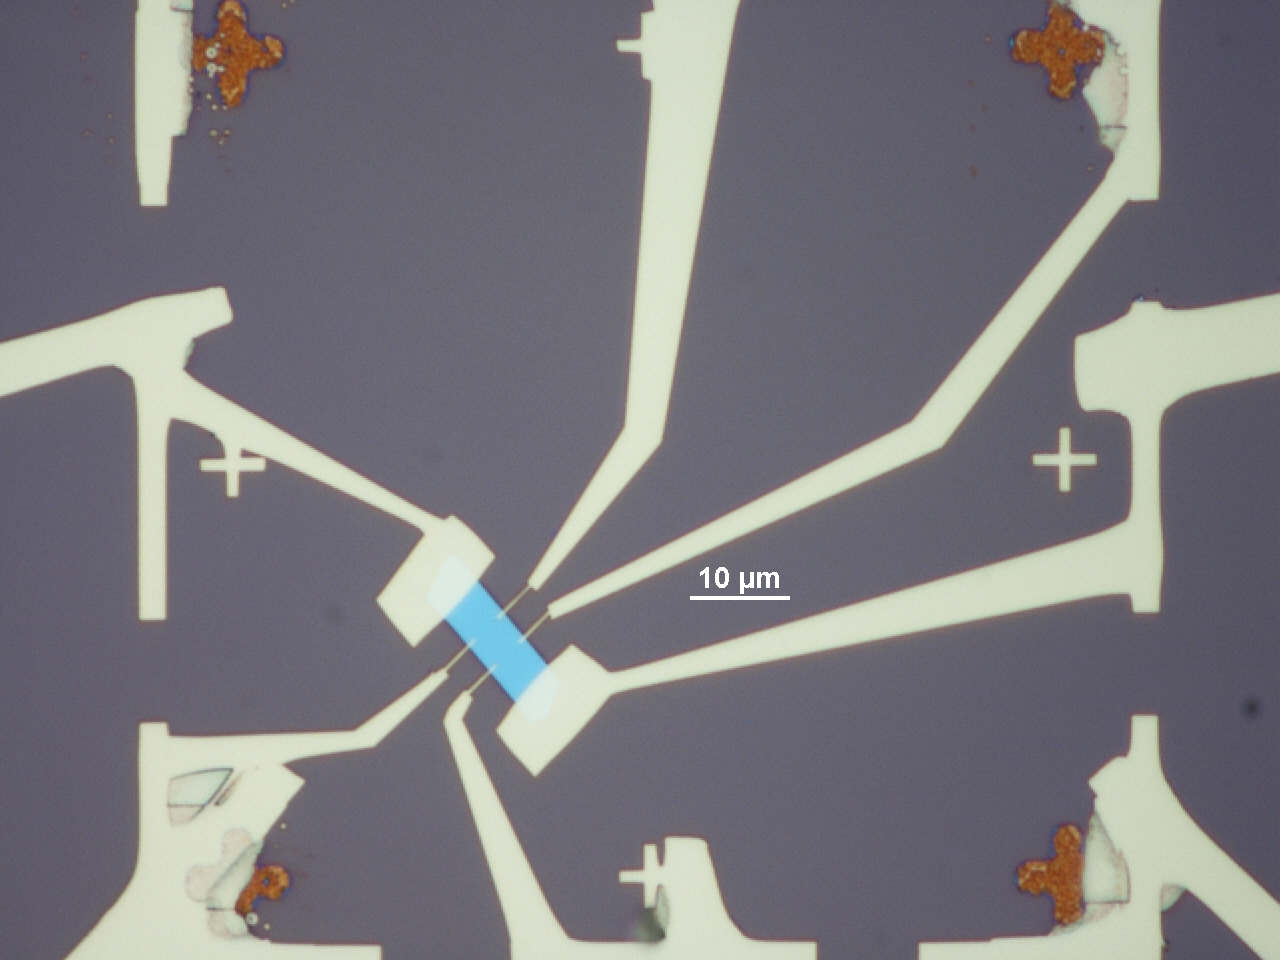
\includegraphics[height=4cm,width=4cm]{figs/experimental/liftoff_100x}
		\label{fig:liftoff_100x}
	}
	\caption[\ch{Au}/\ch{Ti} deposited on device]{Metal deposition on a device pattern.}
\end{figure}


\section{Electrical Measurements}\label{sec:measurements}
\subsection{Measurement Devices}\label{subsec:measurement_devices}
\begin{figure}[ht]
	\centering
	\subfloat[Keithley semiconductor measurement system]{
		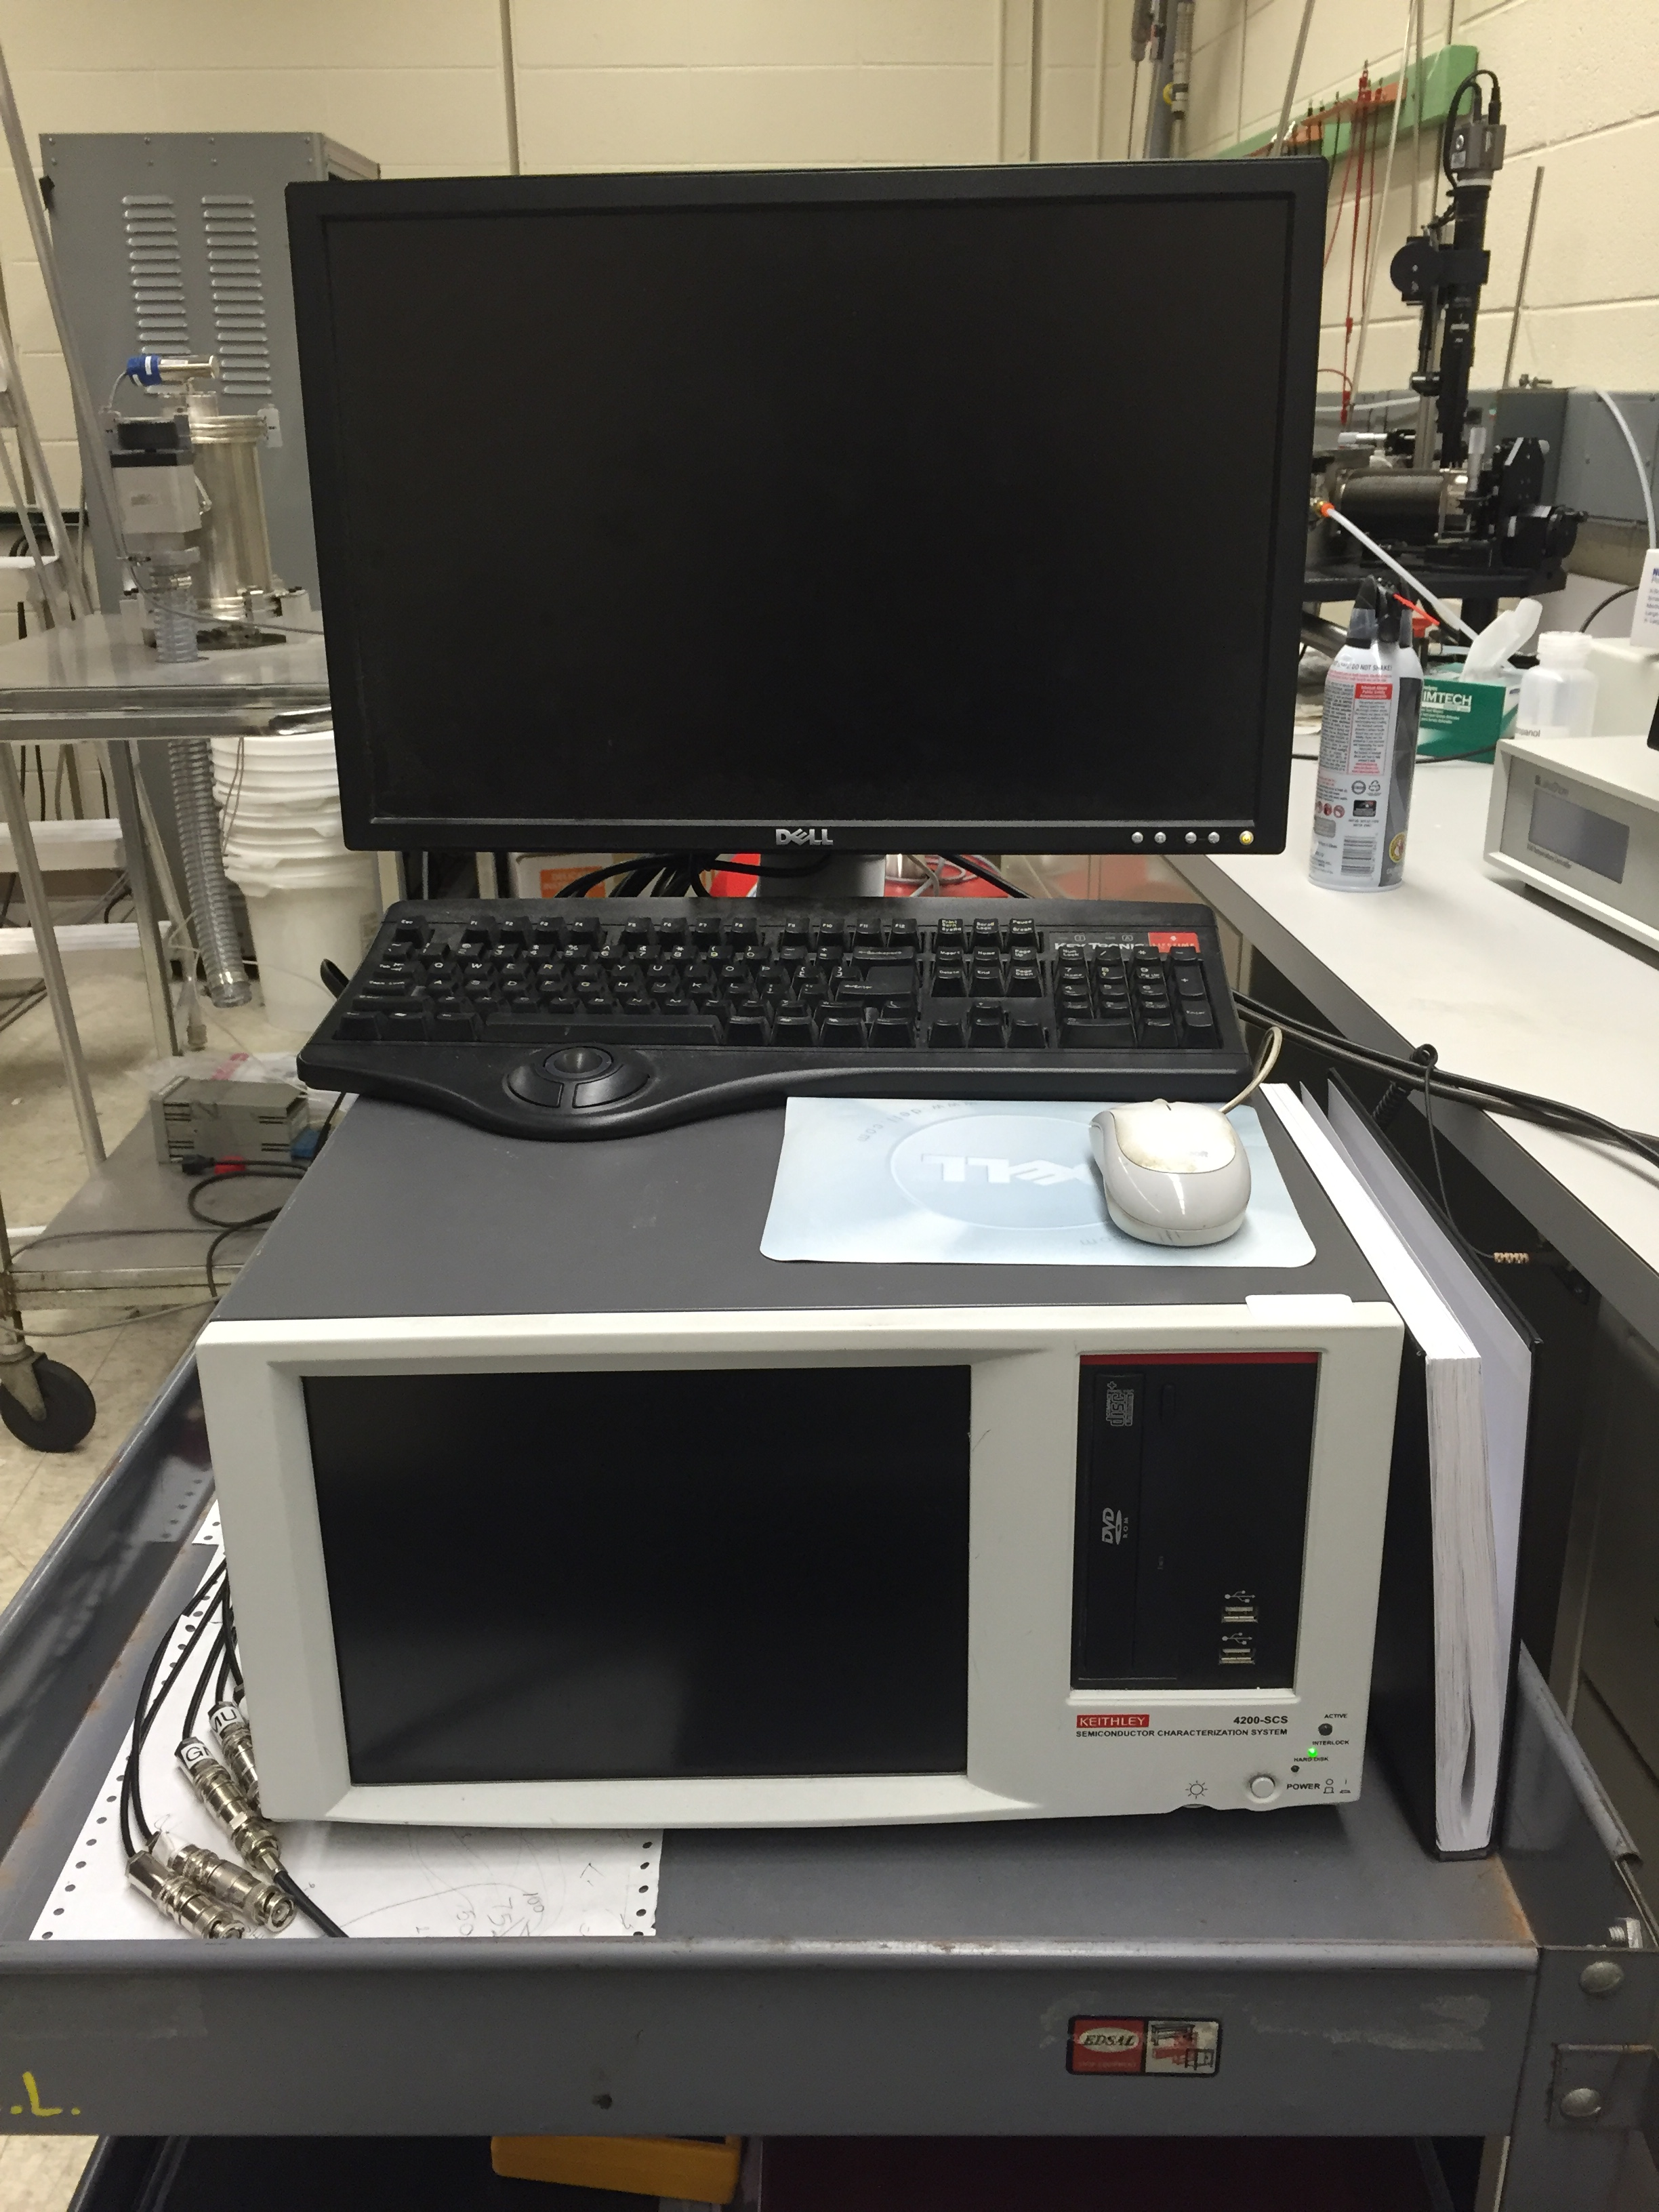
\includegraphics[height=4cm,width=4cm]{figs/experimental/measurement_setup}
		\label{fig:measurement_setup}
	}
	\qquad
	\subfloat[Low temperature, vacuum measurement chamber.]{
		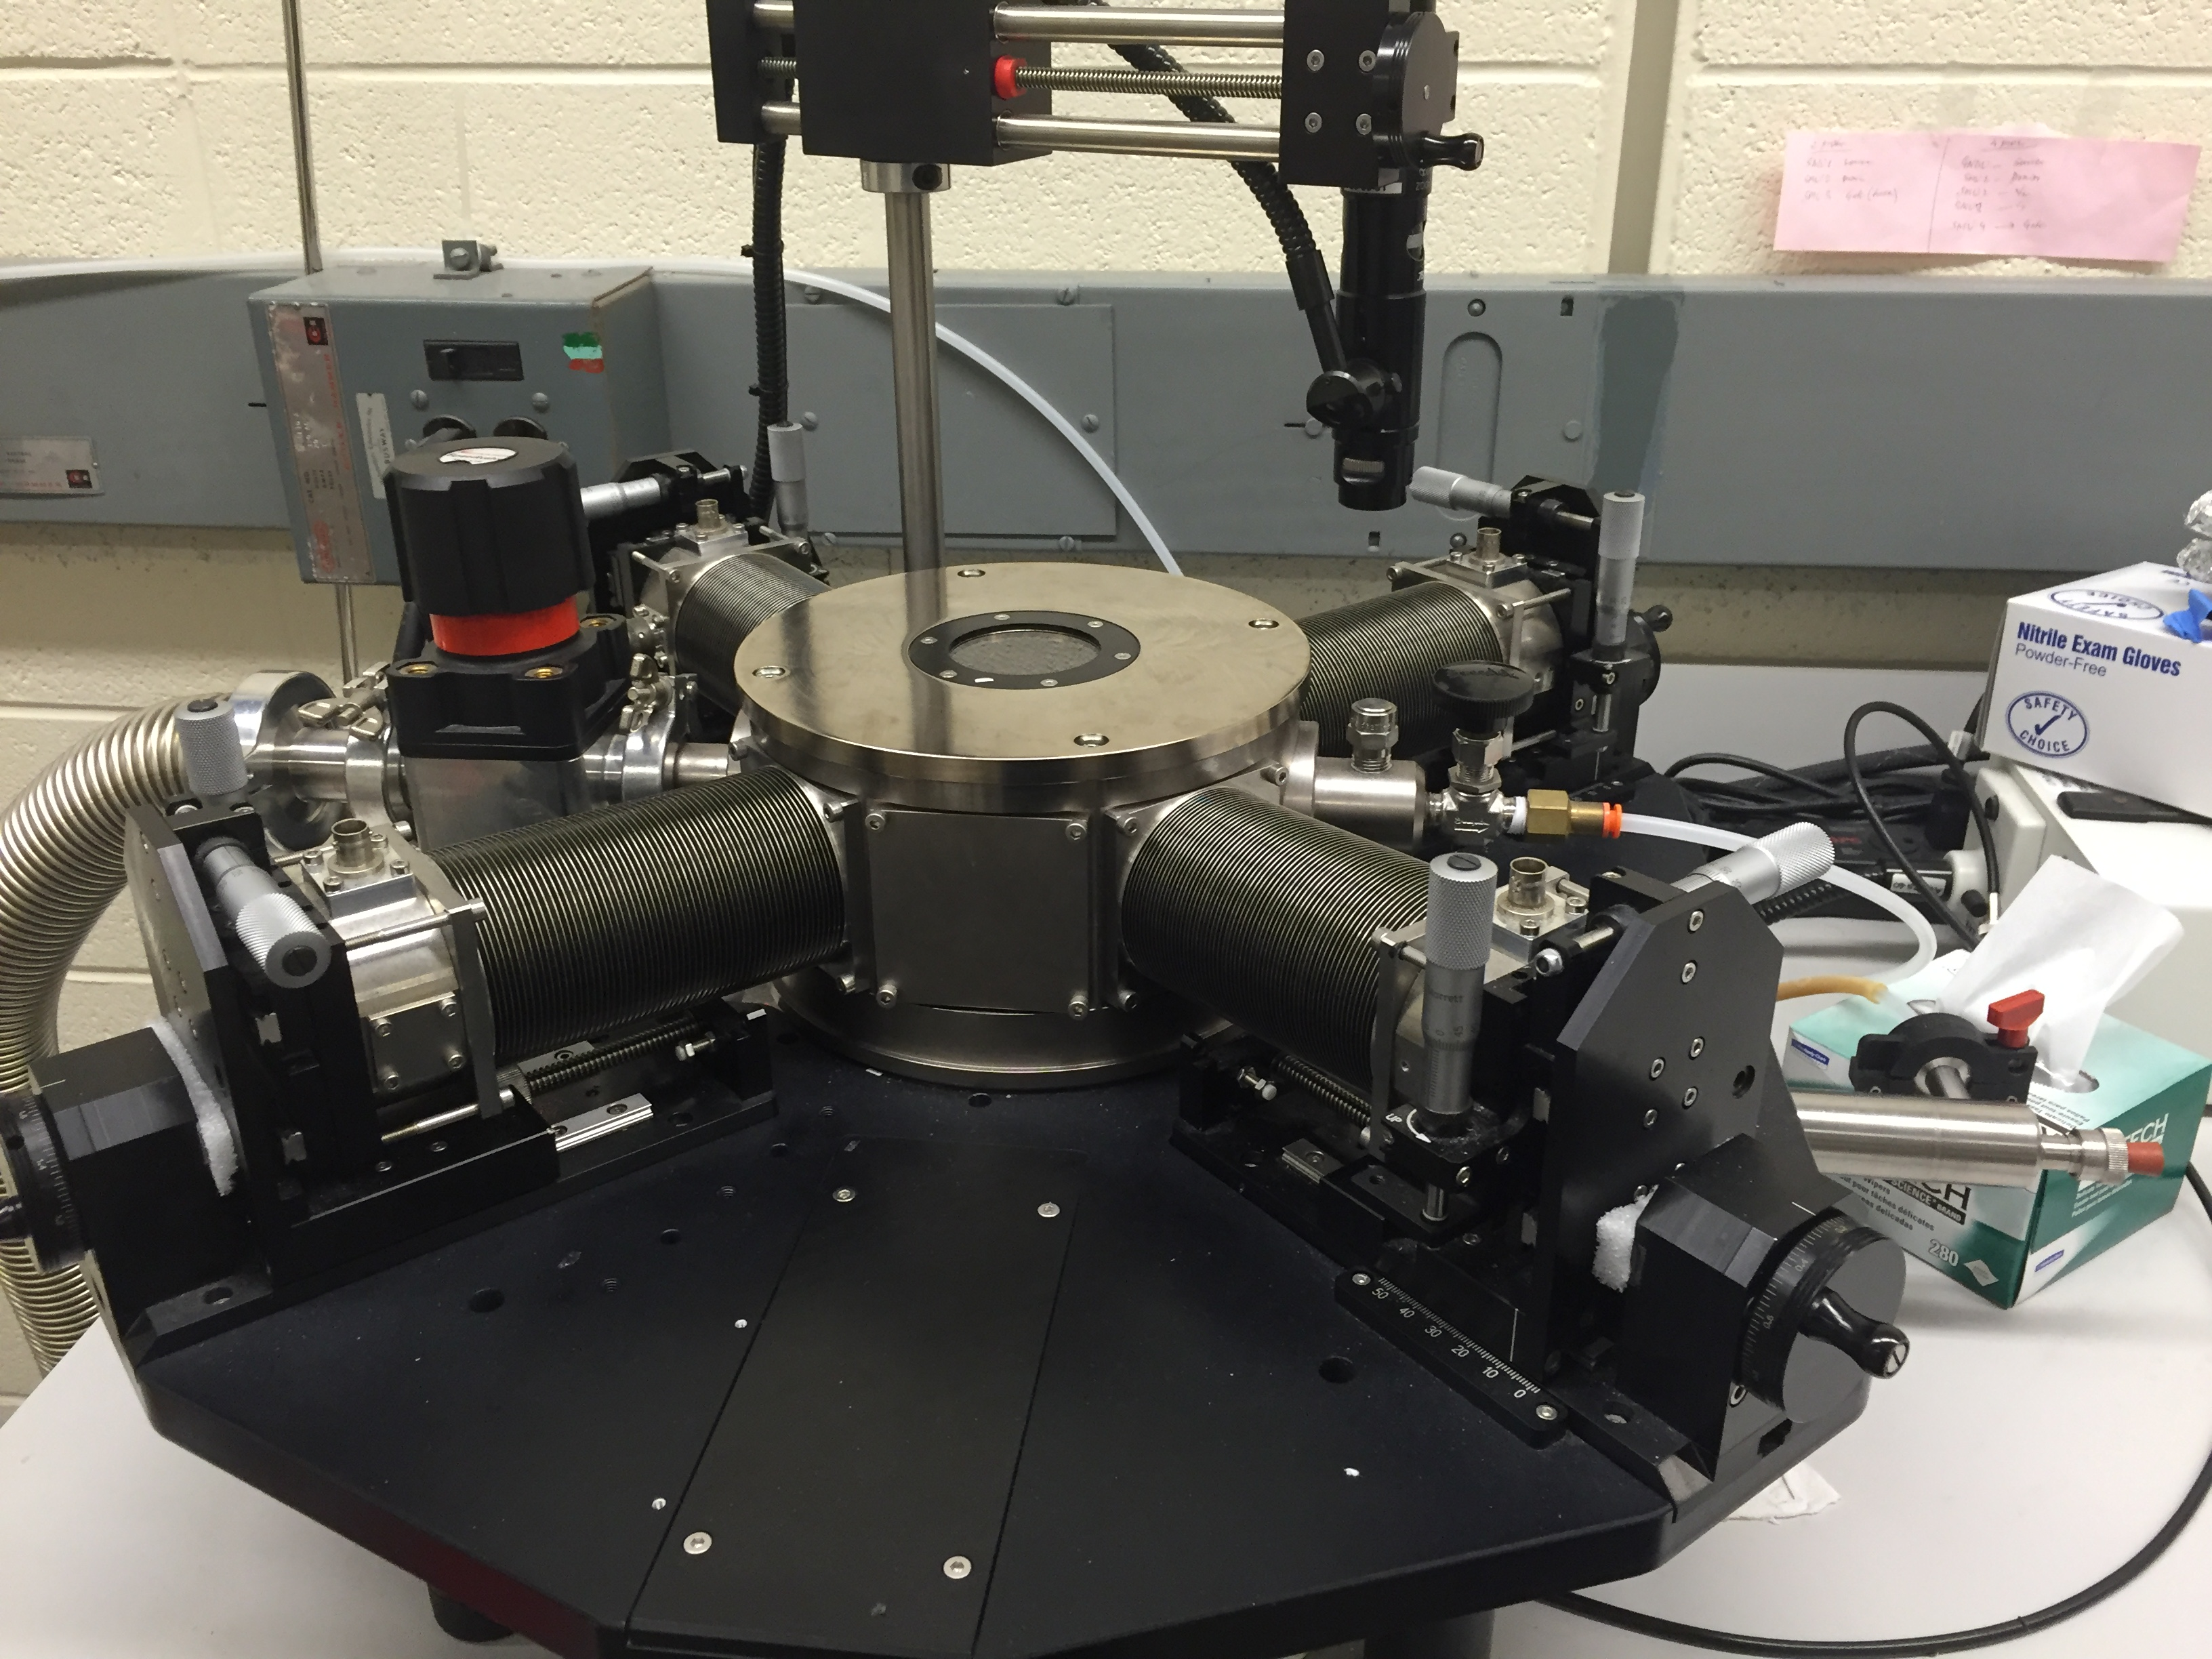
\includegraphics[height=4cm,width=4cm]{figs/experimental/vacuum_measurement}
		\label{fig:vacuum_measurement}
	}
	\caption[Measurement setup]{Main Caption}
	\label{fig:measurement}
\end{figure}

\begin{figure}[ht]
	\centering
	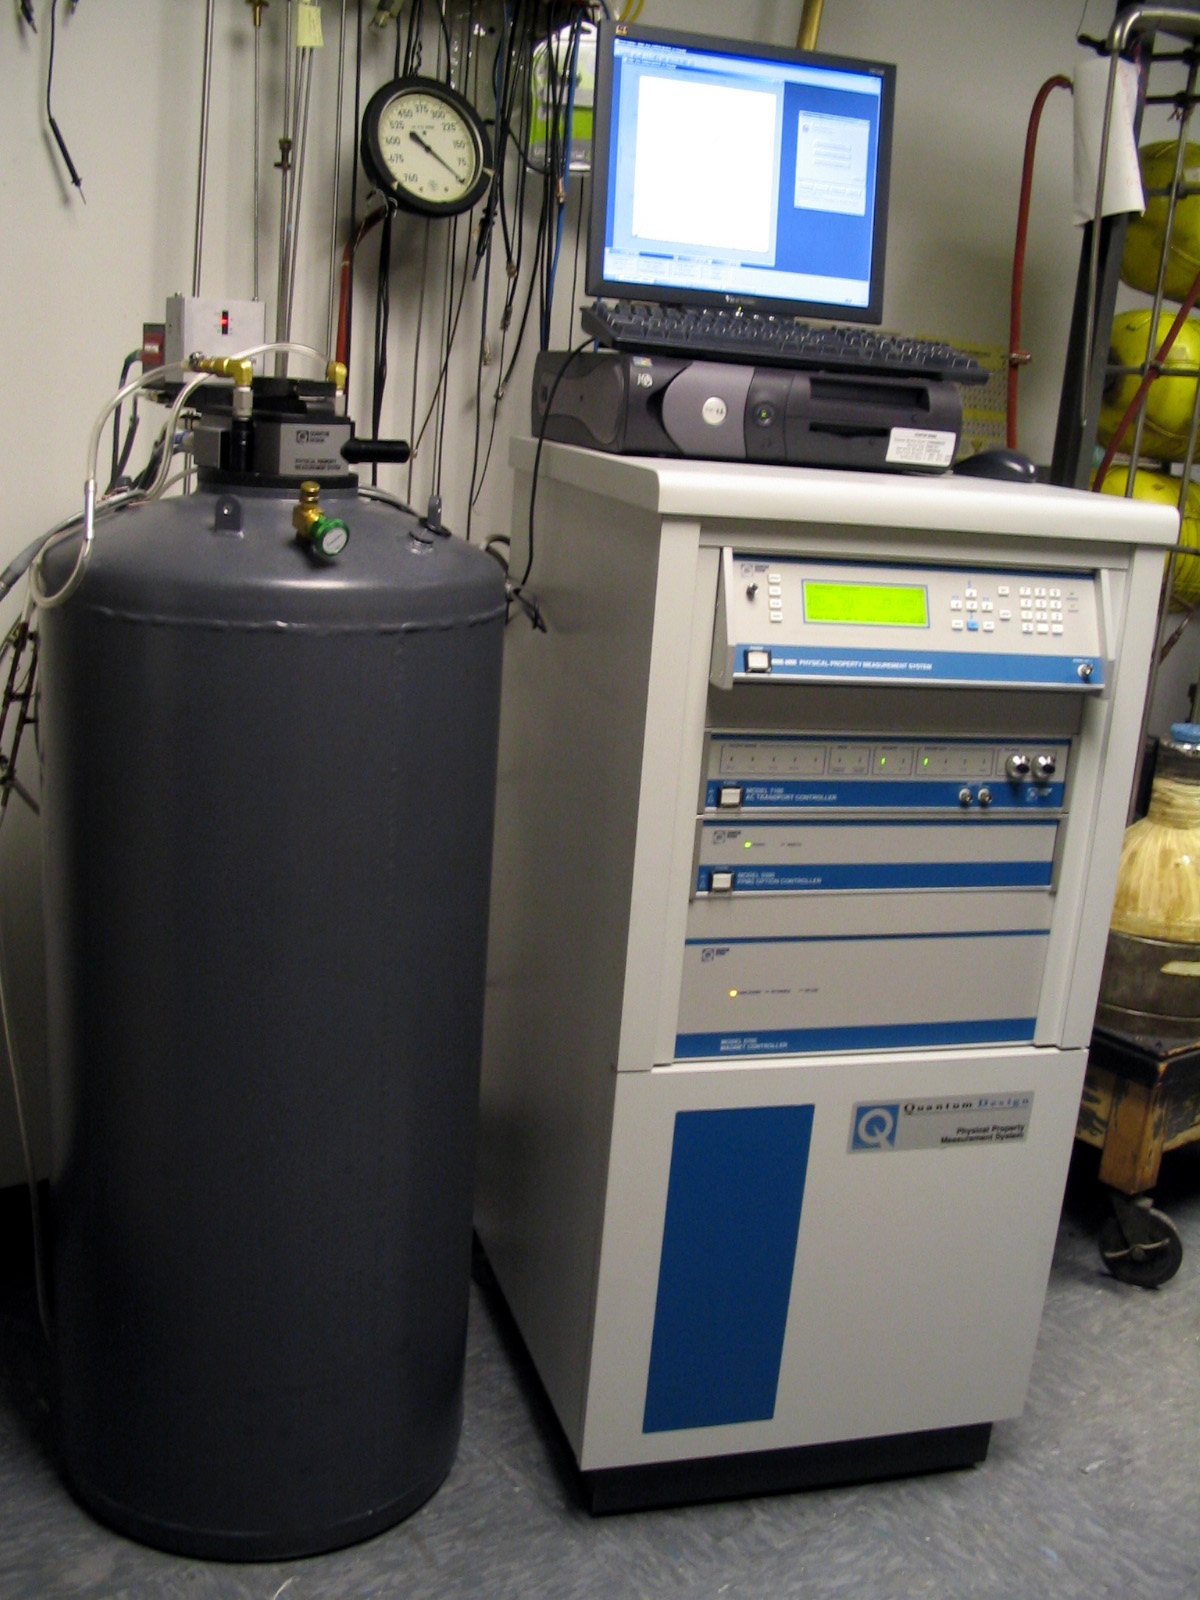
\includegraphics[height=4cm,width=4cm]{figs/experimental/ppms}
	\caption[Physical property measurement system]{\ac{PPMS} for measuring Hall effect and other transport properties.}
	\label{fig:ppms}
\end{figure}

